%---------------------导言区---------------------------%
\documentclass[10pt,a4paper,twoside,UTF8]{ctexart}
\usepackage{geometry}%用于设置上下左右页边距
	\geometry{left=2cm,right=2cm,top=2.5cm,bottom=3cm}
\usepackage{xeCJK,amsmath,paralist,enumerate,booktabs,multirow,graphicx,subfig,setspace,listings}
	\setlength{\parindent}{2em}%正文首行缩进两个汉字
	\lstset{language=tex}
\usepackage{titlesec}
	\newfontfamily\sectionef{Times New Roman}
	\setCJKfamilyfont{FZHeiTi}{黑体}
	\newcommand{\sectioncf}{\CJKfamily{FZHeiTi}}
	\titleformat*{\section}{\large\bfseries\sectioncf\sectionef}
	\titleformat*{\subsection}{\normalsize\bfseries\sectioncf\sectionef}
\usepackage{fancyhdr}
\usepackage{float}
\usepackage{layout}
\setlength{\skip\footins}{0.5cm}%脚注与正文的距离
\renewcommand{\footnotesize}{}%设置脚注字体大小
\setlength\columnsep{0.8cm}%设置双栏的间距
\usepackage{ifthen}%这个宏包提供逻辑判断命令
\newboolean{first}%引入布尔变量
\setboolean{first}{true}%将布尔变量设置为true
\pagestyle{fancy}
	\fancypagestyle{maincontent}{
		\fancyhf{}  %清空页眉页脚设置
		\fancyhead[EL, OR]{\thepage}
		\fancyhead[EC]{实验C6 光纤光学实验}
		\fancyhead[OC]{基\quad 础\quad 物\quad 理\quad 实\quad 验}
		\renewcommand\headrulewidth{0pt}
	}

	\usepackage{datetime}
	\fancypagestyle{firstpage}{
		\setboolean{first}{false}%firstpage出现,则将first重置为false
		\fancyhf{}  %清空页眉页脚设置
		\fancyhead[L]{\the\year 年\the\month 月}
		\fancyhead[R]{\shortmonthname[\the\month], \the\year}
		\fancyhead[C]{
		\large{基\quad 础\quad 物\quad 理\quad 实\quad 验}\\
		\normalsize{GENERAL PHYSICS LABORATORY}
		}
	}

	%%% Step3 页眉线的设置:用布尔变量区分首页和正文
	\newcommand{\makefirstpageheadrule}{%定义首页页眉线-双线绘制命令
	\makebox[0pt][s]{\rule[0.6\baselineskip]{\headwidth}{0.3pt}}
	\makebox[0pt][s]{\protect\hspace{-0.34em}\rule[0.75\baselineskip]{\headwidth}{0.3pt}}
	\protect\vspace{-20pt}
	}

	\newcommand{\makeheadrule}{%定义正文页页眉线绘制命令,单线
	\makebox[0pt][l]{\rule[1\baselineskip]{\headwidth}{0.3pt}}
	\protect\vspace{-20pt}%页眉和正文的距离
	}

	%根据布尔变量first为true或false分别执行不同的页眉线绘制命令
	\renewcommand{\headrule}{%重定义headrule命令
	\ifthenelse{\boolean{first}}{\makeheadrule}
	{\makefirstpageheadrule}
	}
%%end--------------设置首页和正文不同的页眉页脚-----------%%



%%begin-----------------参考文献-----------------------%%
% \usepackage{cite}
% \newcommand{\upcite}[1]{\textsuperscript{\textsuperscript{\cite{#1}}}} %参考文献上标
% \usepackage[backref]{hyperref}
% \usepackage{url}
\usepackage[colorlinks,linkcolor=blue,urlcolor=blue]{hyperref}%超链接
\usepackage[hyperref=true,backend=biber,bibstyle=gb7714-2015,citestyle=numeric-comp,sorting=none,backref=true]{biblatex}
	%hyperref=true和backref=true表示为各个参考文献的引用处、及定理、定义、例子等的引用处都添加上超链接;
	%backend=biber:后端处理的程序为biber.exe
	%bibstyle:参考文献风格;每个期刊、组织要求不同
		%gb7714-2015是目前国内期刊通用的风格,称为gb标准风格
	%citestyle:引用风格;每个期刊、组织要求不同
	%sorting=none:按照参考文献在论文中出现的先后顺序排序。
	%**编译:biblatex与biber命令配合使用。xelatex-biber-xelatex-xelatex
%\addbibresource{ref.bib}
	%这里写上.bib文件的相对地址
	%每次实验引用的页数不同,需要手动改变

%%end-------------------参考文献-----------------------%%
%%%%%%%%%%%%%%%%%%%%%%%%%%%%%%%%%%%%%%%%%%%%%%%%%%%%%%%%%%
%%%%%%%%%%%%%%%%%%%%%%%%%正文开始%%%%%%%%%%%%%%%%%%%%%%%%%%
%%%%%%%%%%%%%%%%%%%%%%%%%%%%%%%%%%%%%%%%%%%%%%%%%%%%%%%%%%

\begin{document}


%%begin-------------------中文摘要-----------------------%%
\title{\LARGE\textbf{实验C6 光纤光学实验}\footnotemark[1]}
\author{\large\textit{XXX\footnotemark[2]}
\\ \normalsize{(1. \textit{中山大学 物理学院,广东 广州 }510275)}}
\date{}%不显示日期


	%twocolumn: 双栏article下的单栏摘要
	\maketitle  %标题和作者
  	\renewcommand{\abstractname} {} %不显示摘要名字
	\begin{abstract}
	\vspace{-3em}
	%vspace:调整垂直空白,可以自己调整;缩小abstract和center(以及maketitle)的间距
	%\noindent %备用:摘要无缩进
	{\bf 摘{} 要:}
	{\small 
	光纤(即光导纤维,optical fiber)是20世纪70年代发展起来的一种新型光电子材料,最初用于通信,70年代末用于传感技术。
	普通光纤由高纯度石英玻璃在高温下拉制而成,有传输损耗低、频带宽、纤径小、重量轻、抗干扰性好、耐腐蚀、耐高温等优点。 
	本次实验采用He-Ne激光器,芯径分别为4$\mu m$、9$\mu m$的单模光纤和芯径为62.5$\mu m$的多模光纤和五维调节架等仪器,首先调节光纤使其与激光器耦合,
	其次测量和计算光纤的数值孔径、耦合效率、耦合损耗等基本属性,初步了解光纤光学。
	实验发现从用同一种耦合方式耦合时,光纤直径越大,其耦合效率越高,传输损耗越低。
	将直接耦合方法与透镜耦合方式比较,透镜耦合的效率显著高于直接耦合,并且传输损耗大大降低。这与透镜聚焦,将光功率汇集于焦点的功能息息相关。
	然后利用光纤马赫-曾德尔干涉仪,分别改变光纤压力或者温度后观察干涉条纹变化,作出干涉条纹随压力或温度变化曲线,线性拟合后发现干涉条纹数与压力或温度均呈线性,
	可用作传感器的制作,通过本实验学习掌握光纤压力传感和光纤温度传感器的设计原理和使用方法。
	最后分别测量线偏振光、圆偏振光和光纤耦合后的水平光功率、垂直光功率,$+45^{\circ}$光功率及圆偏光光功率,并由此计算斯托克斯参数。
	通过一系列实验,可以加深对光纤光学的理解, 提高实验者的综合创新能力。}

	\par%空的新行的高度。
	\textbf{关键词}:光纤、 光纤耦合、 数值孔径、 马赫-曾德尔干涉仪、 光纤传感器、 偏振光
	\vspace{2em}
	\end{abstract}

%%end--------------------英文摘要------------------------%%
\renewcommand{\thefootnote}{\fnsymbol{footnote}}
\footnotetext[1]{由中山大学物理学院陆佑堂提供器材和指导。}
\footnotetext[2]{作者简介:XXX,xxxxxxxx;E-mail: \url{xxxxx@mail2.sysu.edu.cn}}

%%end-------------------中文摘要-----------------------%%


\thispagestyle{firstpage}%首页页面风格:firstpage
\pagestyle{maincontent}%第二页之后的页面风格:maincontent

%%begin------------------英文摘要------------------------%%

	\renewcommand{\abstractname} {} %不显示摘要名字
	\begin{center}%
		\begin{spacing}{2.0}
			{\LARGE\bfseries Experiment C6: Optical Fiber Experiment$^{*}$  }%
		\end{spacing}
	    \vskip 0.5em%
	    {\large
	    \lineskip .75em%
	    \begin{tabular}[t]{c}%
	    \large XXX$^{1}$
	    \end{tabular} 
	    }%
	    \vskip 0.4em%
	    {\normalsize 1. School of Physics, Sun Yat-sen University, Guangzhou  { \rm 510275}, China}
	\end{center}
	\begin{abstract}
		\vspace{-2em}  %缩小abstract和center(以及maketitle)的间距
	    	{\bf Abstract:}
	    {\small 
		Optical fiber is a new type of optoelectronic material developed in the 1970s. It was originally used for communication and sensing in the late 1970s.  
		Common optical fiber is made of high purity quartz glass under high temperature, which has the advantages of low transmission loss, wide frequency band, small fiber diameter, light weight, good anti-interference, corrosion resistance, high temperature resistance and so on.  
		In this experiment, we used He-NE laser, single mode fiber with core diameter of 4$\mu m$, 9$\mu m$, multi-mode fiber with core diameter of 62.5$\mu m$ and five-dimensional adjusting frame. 
		Firstly, the fiber was adjusted to couple with the laser.  
		Secondly, the numerical aperture, coupling efficiency, coupling loss and other basic properties of the optical fiber are measured and calculated.  
		It is found that the larger the fiber diameter is, the higher the coupling efficiency and the lower the transmission loss are when the fiber is coupled in the same coupling mode.  
		Compared with the direct coupling method, the efficiency of the coupling method through lens is significantly higher than that of the direct coupling method, and the transmission loss was greatly reduced.  
		This is closely related to the ability of the lens to focus light power at the focal point.  
		Then, the fiber Mach-Zehnder interferometer was used to observe the change of interference fringes after changing the pressure or temperature of the fiber respectively, and the curve of interference fringes changing with the pressure or temperature was made. 
		After linear fitting, it was found that the number of interference fringes was linear with the pressure or temperature.  
		Then we drew the conclusion that optical fiber can be used as a sensor. Through this experiment, we can learn the design principle and use method of optical fiber pressure sensor and optical fiber temperature sensor.  
		Finally, the horizontal optical power, vertical optical power, $+45^{\circ}$ optical power and circularly polarized optical power after the coupling of linearly polarized light, circularly polarized light and fiber are measured respectively.
		Then we used these four parameters to calcuklate Stokes parameter.
		Through a series of experiments, we can deepen the understanding of fiber optics and improve the comprehensive innovation ability of this experimenter.  		}
	    \par%空的新行的高度。
		\textbf{Key words}:optical fiber, fiber coupling, numerical aperture, Mach-Zehnder interferometer, fiber sensor, polarized light     
	\end{abstract}
	~\\



%%begin----------------层级结构------------------------%%

%重点1:知道每一个层级的样式和怎么和后面的正文接上
%重点2:掌握各种换段的方法
%重点3:自定义的项目符号(宏包enumerate的用法)

\section{引 \quad 言}
光纤(即光导纤维,optical fiber)是 20 世纪 70 年代发展起来的一种新型光电子材料,最初用
于通信,70 年代末用于传感技术。普通光纤由高纯度石英玻璃在高温下拉制而成,有传输损耗低、频带宽、纤径小、重量轻、抗干扰性好、耐腐蚀、耐高温等优点。
用光纤作为激光的传输介质,搭建激光干涉光路,并通过干涉条纹随光纤所受外作用(如温度、应变等)而变化的情况可以实现传感器的功能。
通过本实验可以认识斯托克斯参数对偏振测量的意义和认识光纤传输的偏振模色散,并且测量偏振光的斯托克斯参数,测量了光纤传输后偏振状态的改变情况。

\section{介 \quad 绍}
\subsection{光纤耦合}
\subsubsection{光纤的传播模式}
光波在光纤中的传播,主要是交变的电场和磁场在光纤中向前传播。电磁场的各种不同分布形
式,称为“模式”(mode)。任何在光纤中传输的光波必须满足在纤芯和包层界面上应用 Maxwell
波动方程的边界条件,其结果是,光纤中的光波只能形成独特的一个或多个模式。单模光纤是只能
传输一种模式的光纤,在光纤的横截面上只存在一种电磁场分布模式;而多模光纤能传输多个模
式,在光纤横截面上允许多个电磁场分布模式同时存在。光纤内传输模式的总数由一个无量纲的参
数----归一化频率 V 决定,
\begin{equation}
	\label{eq:1}
	V=2\pi a n_1 \frac{\sqrt{2\varDelta}}{\lambda}
\end{equation}
其中$\varDelta=(n_1-n_2)/n_1$,称为相对折射率差;a 为纤芯半径;$\lambda$为光波长。在归一化频率 V 较大的情
况下,传输模式总数约为$\frac{V^{2}}{2}$(阶跃型)-$\frac{V^{2}}{4}$(梯度型)。由光波动理论可以证明,对于特定的波长$\lambda$,
当V < 2.405 时,单模传输条件成立。此时,入射光中只有一个模式(即基模)能够在光纤中传
播。为满足单模的条件,光纤纤芯直径 2a 都很小,约为 2-12$\mu m$,包层直径 2b 约 125$\mu m$;而多
模光纤的芯径 2a 较大,典型值为 50$\mu m$。从两种光纤的性质比较来看,单模光纤的信号传输性能较
好,传输容量大,但不易耦合、制造,连接工艺复杂,传输的光能量低。多模光纤的信号传输性能
差,传输容量小,但耦合、制造和连接相对容易,因此传输的光能量也较大。

\subsubsection{光纤的数值孔径}
在均匀折射率光纤中,光是依靠在纤芯和包层两种介质分界面上的全反射向前传播的。射入光
纤的光线有两种,一种是穿过光纤纤芯轴线的光线,叫子午光线,如图\ref{fig:1}所示,子午光
线在光纤内沿锯齿形的折线前进。另一种是弧矢光线,不穿过纤芯的轴线,如图\ref{fig:2}所
示,从光纤的横剖面上看,弧矢光线的传播轨迹呈多边形折线状。
\begin{figure}[H]
	\centering
	\subfloat[子午光线]{\label{fig:1}
	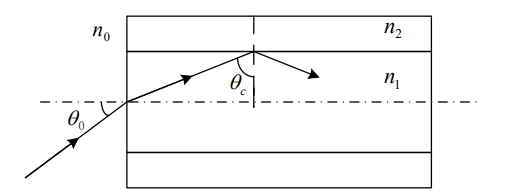
\includegraphics[width=0.5\textwidth]{img/1.png}
	}
	\subfloat[弧矢光线]{\label{fig:2}
	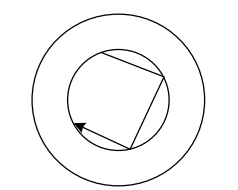
\includegraphics[width=0.3\textwidth]{img/2.png}
	}
	\caption{均匀折射率光纤中光线的传播}
	\label{fig:total1}
\end{figure}

如图 \ref{fig:1},设光线在光纤端面上的入射角为$\theta$(光线从空气进入折射率为$n_1$的纤芯),
设光线在纤芯与包层分界面处的入射角为$\theta_i$。对于子午光线,$\theta_i$应满足全反射条件,
\begin{equation}
	\label{eq:2}
	\theta_i >\theta_c =arcsin\left(\frac{n_2}{n_1}\right)
\end{equation}

其中$\theta_c$为全反射临界角。故光纤端面外侧入射的光束存在一个最大入射孔径角$\theta_0$,入射角大于$\theta_0$的
光线在纤芯与包层界面不再满足全反射条件而无法在光纤中稳定传输。由折射定律及式\ref{eq:2}可得:

\begin{equation}
	 n_0 sin \theta_0 = n_1 sin (\frac{\pi}{2}-\theta_c)=n_1 cos\theta_c =\sqrt{n^{2}_1-n^{2}_2}
\end{equation}

\begin{equation}
	\theta_0=arcsin(\frac{1}{n_0}\sqrt{n^{2}_1-n^{2}_2})
\end{equation}
入射角$\theta$小于$\theta_0$的子午光线,都可以在光纤中靠全反射向前传输。入射角大于$\theta$的子午光线在界面
上发生折射穿过包层射出,不能向前传输。

$n_0 sin \theta_0 $是反映光纤性能的一个重要参数,称为光纤的数值孔径 NA(Numerical Aperture)。它
表示光纤收集光的本领及与光源耦合的难易程度。光纤的 NA 大,收集、传输能量的本领就大。若
将纤芯与包层的相对折射率差用
$\varDelta=\frac{(n_1-n_2)}{n_1}=1-\frac{n_2}{n_1}$
表示,则数值孔径可表示为:
\begin{equation}
	NA=n_0 sin\theta_0 =\sqrt{n^{2}_1-n^{2}_2}\approx n_1 \sqrt{2\varDelta}
\end{equation}

光纤数值孔径的另一种定义是远场强度有效数值孔径,它是通过测量光纤远场强度分布来确定
的。其定义方法是:当远场辐射强度(每单位立体角的光功率)达到稳态分布时,测量光纤出射端
的光功率分布曲线以及光纤端与探测界面的距离,光强下降到最大值的 5\%处的半张角的正弦值即
为光纤的数值孔径,有:
\begin{equation}
	NA_{max}= \frac{q}{\sqrt{q^2+l^2}}
	\label{eq:NA}
\end{equation}

采用上述方法测量光纤的数值孔径,待测光纤不宜太长或太短,以 2m 左右为宜。

\begin{figure}[H]
	\centering
	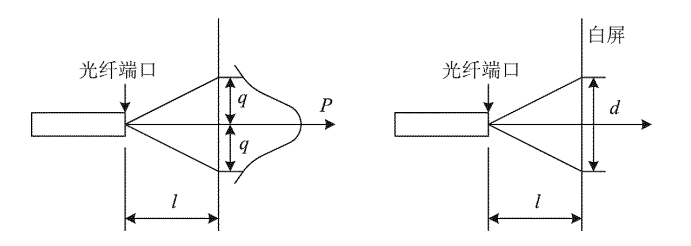
\includegraphics[width=0.8\textwidth]{img//3.png}
	\caption{远场光强法和远场光斑法原理图}
	\label{fig:3}
\end{figure}

光纤数值孔径的测量方法:
\begin{enumerate}
	\item 远场光强法
	
	远场光强法是 CCITT 组织规定的 G.651 多模光纤的基准测试方法.该方法对测试光纤样品的处
	理有严格要求,需要强度可调的非相干稳定光源,具有良好线性的光检测器等等。
	\item 远场光斑法

	这种测试方法的原理本质上类似于远场光强法,只是结果的获取方法不同。简单易行,可以采
	用相干光源,原理性实验中多采用这种方法,如图\ref{fig:3}所示。测量时,在暗室中将光纤出
	射远场投射到白屏上,测量光斑直径 d,用光斑半径 d/2 替代远场强度法中的 q 值,测量光纤端与
	观察屏的距离 l,然后用式\ref{eq:NA}计算光纤的最大理论数值孔径。	
\end{enumerate}

\subsubsection{光纤与光源的耦合}
光纤与光源的耦合有直接耦合和经聚光器件耦合两种。直接耦合是使光纤直接对准光源输出的
光进行的对接耦合。将制备好的光纤端面靠近光源的发光面,调整两者的相互位置,使光纤输出端
的输出光强最大,然后固定该相对位置。这种方法简单可靠,但必须有专用设备。如果光源输出光
束的横截面积大于纤芯的横截面积,将引起较大的耦合损耗。

经聚光器件耦合是将光源发出的光通过聚光器件聚焦到光纤端面上,并调整到最佳位置,使光
纤输出光强最大,这种方法耦合效率较高。聚光器件有传统的透镜和自聚焦透镜。
耦合效率的计算公式为:

\begin{equation}
	\eta=-10log \left(\frac{P_1}{P_2}\right) (dB)
\end{equation}

其中$P_1$为耦合进光纤的光功率(近似为光纤的输出光功率),$P_2$为光源输出的光功率。

\subsubsection{激光与光纤的耦合损耗}
目前在激光与光纤的耦合技术中,主要还是以机械结构来控制光束与光纤的相对位置。导致耦
合效率下降的原因主要有三种机械对准误差:横向、纵向、角向。

横向偏移误差 d 是指光斑中心和纤芯中心没有完全重合而产生的误差。如图 \ref{fig:4} 所示,其
中 R 和$\omega$分别为光纤纤芯半径和聚焦激光光斑半径。两中心由于存在横向偏移 d,使得部分光束照
射不到光纤端面,产生损耗。

\begin{figure}[H]
	\centering
	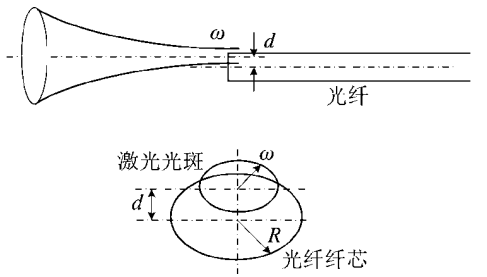
\includegraphics[width=0.5\textwidth]{img//4.png}
	\caption{横向偏移误差的示意图}
	\label{fig:4}
\end{figure}

纵向偏移误差是指轴线方向上聚焦光斑和光纤端面之间的距离不匹配,使光斑在光纤端面处的
面积大于光纤纤芯端面的面积而产生损耗。如图\ref{fig:5}所示,$\omega$为聚焦激光光斑半径,s 为聚焦
光斑与光纤端面的距离。假设聚焦后的光斑直径等于光纤芯径,则存在纵向偏移误差时光纤耦合效
率正比于纤芯端面面积和端面处的光束面积之比。

\begin{figure}[H]
	\centering
	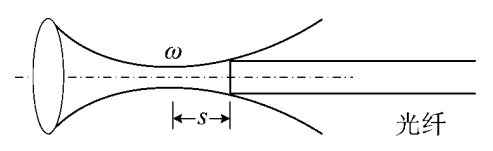
\includegraphics[width=0.5\textwidth]{img//5.png}
	\caption{纵向偏移误差示意图}
	\label{fig:5}
\end{figure}

角度偏移误差是指聚焦光束光轴与光纤光轴不重合而产生的误差。图\ref{fig:6} 所示,两光轴存
在夹角𝜃将导致聚焦光束发散角与光纤数值孔径不匹配,即不满足耦合条件中角度条件
($\theta_{laser}<2 arcsin(NA)$),使光纤损失掉置于最大接收立体角之外的光功率。光纤端面和光纤轴不是严
格正交,也会损失掉部分不满足全反射条件的光。

\begin{figure}[H]
	\centering
	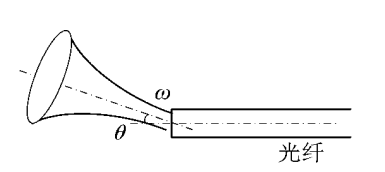
\includegraphics[width=0.5\textwidth]{img//6.png}
	\caption{ 角度偏移误差示意图}
	\label{fig:6}
\end{figure}

\subsubsection{光纤的传输损耗}
光波在光纤中传输,随着传输距离的增加,光波强度(或光功率)将逐渐减弱,这就是传输损
耗。光纤的传输损耗与所传输的光波长$\lambda$相关,与传输距离L成正比。通常以传输损耗系数$\alpha(\lambda)$
表示损耗的大小。光纤的损耗系数为光波在光纤中传输单位距离所引起的损耗,常以短光纤的输出
光功率 $P_1$和长光纤的输出光功率 $P_2$之比的对数表示,即

\begin{equation}
	\alpha\left(\lambda\right)=\frac{1}{L} 10 lpg \frac{P_1}{P_2} (dB)
	\label{eq:eff}
\end{equation}

光纤的传输损耗是由许多因素引起的,有光纤本身的损耗和使用条件造成的损耗。光纤传输损
耗测量的方法有截断法、介入损耗法和背向散射法等。

\begin{enumerate}
	\item 截断法
	
	直接利用光纤传输损耗系数的定义的测量方法,是 CCITT 组织规定的基准测试方法。在不改
变输入条件下,分别测出长光纤的输出光功率和剪断后约为 2m 长的短光纤的输出光功率,按传输
损耗系数的表示式\ref{eq:eff}计算出$\alpha(\lambda)$。这种方法测量精度最高,但它是一种“破坏性”的方法。

    \item 介入损耗法
    
	原理上类似于截断法,只不过用带活动接头的连接线替代短光纤进行参考测量,计算在预先相
互连接的注入系统和接收系统之间(参考条件)由于插入被测光纤引起的光功率损耗。显然,光功
率的测量没有截断法直接,而且由于连接的损耗会给测量带来误差。因此这种方法准确度和重复性
不如截断法。

    \item 背向散射法

	通过光纤中的后向散射光信号来提取光纤传输损耗的一种间接的测量方法。只需将待测光纤样
	品插入专门的仪器就可以获取损耗信息。不过这种专门仪器(光时域反射计—OTDR)价格昂贵。
\end{enumerate}


\subsection{光纤传感器}
\subsubsection{光纤马赫-曾德干涉仪}
英国物理学家托马斯·杨最初所作的双缝干涉实验如图 \ref{fig:7} 所示,由光源 L 发出的光照射
在单缝 S 上,使 S 成为一个线光源,在 S 后面放置两个相距很近的狭缝 $S_1$和 $S_2$,且两者与 S 之间的
距离相等。由于$S_1$和 $S_2$是由同一光源 S 的球形波阵面上分离出来的两个光源,满足振动方向、频
率相同,相位差为零的相干条件,所以两者发出的光在空间相遇,将产生如图 \ref{fig:8} 所示的干涉
条纹。

\begin{figure}[H]
	\centering
	\subfloat[杨氏双缝干涉实验原理图]{\label{fig:7}
	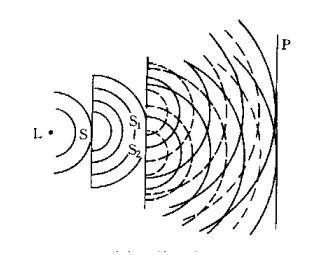
\includegraphics[width=0.4\textwidth]{img/7.png}
	}%
	\subfloat[双光纤干涉条纹]{\label{fig:8}
	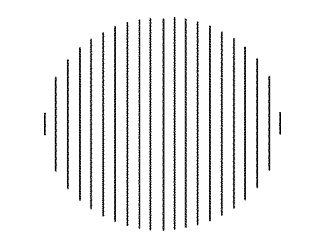
\includegraphics[width=0.4\textwidth]{img/8.png}
	}%
	\caption{}
\end{figure}

采用光纤传输激光,用光纤输出端作为产生相干光的光源来实现双缝干涉,也可以获得干涉图
样。双光路光纤马赫-曾德(Mach-Zehnder,简称 M-Z)干涉仪的工作原理如图\ref{fig:9}所示,从激
光器输出的激光经透镜耦合后进入光纤,经分路器被分为两路,经过两根光纤出射后光场在空间发
生干涉,形成如图\ref{fig:8}所示的均匀干涉条纹。

由双光束干涉的原理可知,干涉场的干涉光强为:
\begin{equation}
	I \propto  1+cos\delta
	\label{eq:9}
\end{equation}

其中$\delta$为干涉仪两臂的光程差对应的位相差,$\delta$等于 2$\pi$的整数倍时为干涉场为极大值。两光纤所构
成的光路受到干扰时,会导致空间干涉条纹的移动。利用这一特性,可以构成光纤 M-Z 干涉仪传感
器。经分路器后的两条光纤,一根作为参考光纤,一根作为传感器的相位调制光纤。当后者受到干
扰,光程发生改变,即相位差发生改变,该变化可按式\ref{eq:9}的规律表现出来。

\begin{figure}[H]
	\centering
	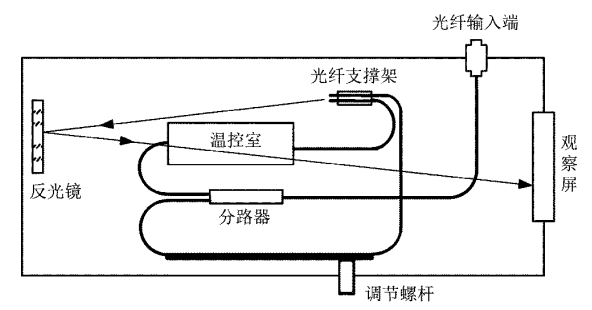
\includegraphics[width=0.7\textwidth]{img//9.png}
	\caption{M-Z光纤干涉仪原理图}
	\label{fig:9}
\end{figure}

\subsubsection{光纤应变传感器}
原理如图\ref{fig:10}所示,光经过一段光纤后光波的相位为$\phi = \beta L$。光纤应变导致输出光的相位变
化量可表示为

\begin{equation}
	\varDelta \phi = L \varDelta \beta + \beta \varDelta L
	\label{eq:10}
\end{equation}

其中$\beta$是光在单模光纤中的传播常数,式\ref{eq:10}右边第一项表示应变引起的效应。第二项表示$\beta$变化
引起的效应,它主要由两个因素导致:应变光效应(即应变改变了光纤的折射率)和波导模色散效
应(应变使光纤直径发生变化)。

\begin{figure}[H]
	\centering
	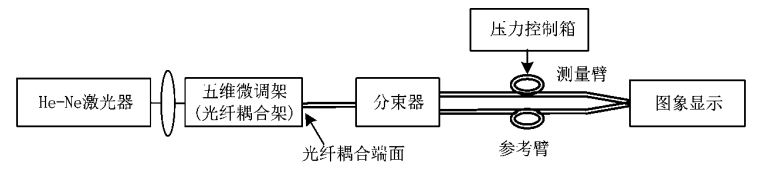
\includegraphics[width=0.9\textwidth]{img//10.png}
	\caption{光纤压力传感原理示意图}
	\label{fig:10}
\end{figure}


\subsubsection{光纤温度传感器}
光纤受热后发生线性热膨胀,长度 L 改变;温度的变化还会导致光学折射率 n 发生变化,两
种因素均会导致光相位发生变化。利用该原理可实现对温度的传感。光经过一段光纤后光波的相
移为$\phi = 2\pi nL/\lambda$,可写成
\begin{equation}
	\frac{\varDelta \phi}{\varDelta T L}=\frac{2\pi}{\lambda}\left(\frac{n}{L}\frac{dL}{dT}+\frac{dn}{dT}\right)
\end{equation}

\begin{figure}[H]
	\centering
	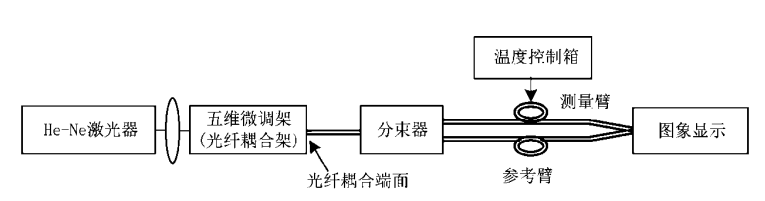
\includegraphics[width=0.9\textwidth]{img//11.png}
	\caption{光纤温度传感原理示意图}
	\label{fig:11}
\end{figure}

\subsection{光纤偏振光}
\subsubsection{偏振态的描述}
1852 年,英国科学家斯托克斯(George Gabriel Stokes,1819~1903)提出用一组可
测量的参数表示光波的偏振态,称为光学偏振的斯托克斯参量表示。对光的偏振有多
种其他表示方法,如琼斯矩阵用光波的每个电场强度分量表示偏振态,但由于光波的
电场强度是随光频变化的快变量,目前的探测器无法响应如此高频的变化,故琼斯矩
阵被认为是不可测量量;又如用相干矩阵表示偏振态,但由于其对角元一般为复数,
所以其矩阵元也被认为是不可测量量。斯托克斯参量的优点是可以直接测量,而且人
们已经认识到这种表示的意义不仅仅是提供一种可测量的表示方法,还成为了连接光
波的经典图像和量子图像的桥梁。

如图\ref{fig:11}所示,设沿着 z 方向传播的偏振光的两个电场分量为

\[\left\{
\begin{aligned}
&E_x= a_1 cos\tau \\
&E_y= a_2 cos(\tau+\delta) \\
\end{aligned}
\right.
\]

其中$a_1$和$a_2$是两个分量的振幅,$\delta$是两个分量的相位差,$\tau(=\frac{2\pi z}{\lambda}-\omega t)$为传播变量。通
过三角变换消去两式中的$\tau$后合成为一个方程

\begin{equation}
	\left(\frac{E_x}{a_1}\right)^2+\left(\frac{E_y}{a_2}\right)^2-\frac{2E_x E_y}{a_1 a_2} cos\delta= sin^{2} \delta
\end{equation}

这样就得到一个关于$E_x$和$E_y$两个变量的非标准形式椭圆方程。对于 z 轴上固定的一点,
𝐸𝑥和𝐸𝑦合成的电场矢量顶点在$E_x-E_y$平面内以椭圆轨迹做旋转运动,如图\ref{fig:12}所示,
被称为偏振椭圆。电场向前传播时,电场矢量顶点在三维空间中的椭圆柱面上描绘出
一条螺旋轨迹\ref{fig:13}。

\begin{figure}[H]
	\centering
	\subfloat[在垂直 Z 轴横截面上的轨迹]{\label{fig:12}
	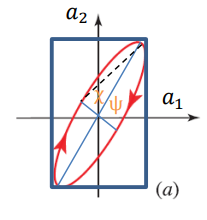
\includegraphics[width=0.2\textwidth]{img/12.png}
	}%
	\subfloat[三维空间轨迹]{\label{fig:13}
	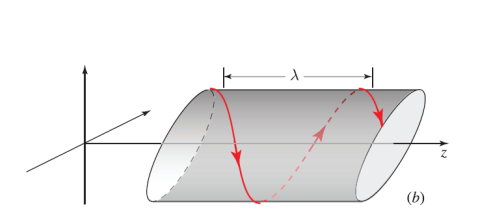
\includegraphics[width=0.5\textwidth]{img/13.png}
	}%
	\caption{椭圆偏振光电场矢量顶点轨迹}
\end{figure}

偏振椭圆内接于一长方形,长方形的边与坐标轴平行,边长为$2a_1$和$2a_2$(见图\ref{fig:14}),
椭圆和各边相切于点$(\pm a_1,\pm a_2 cos \delta )$和$(\pm a_1 cos \delta,\pm a_2)$。这样可用两个角度表征偏振
状态:方位角$\psi (0< \psi < \pi /2)$确定椭圆的方向,它是长轴和$E_x$轴的夹角;表征椭圆率
以及椭圆转向的$\chi $角$(-\pi /4< \chi< \pi/4)$确定椭圆的形状和转向
\begin{equation}
	\mp \frac{b}{a} = tan \chi
\end{equation}
$\psi$和$\chi$都取决于两个分量的振幅和相位差:
\[\left\{
\begin{aligned}
&	tan (2\psi)=\frac{2a_1 a_2}{a^2_1-a^2_2}cos\delta \\
&	tan (2\chi)=\frac{2a_1 a_2}{a^2_1+a^2_2}sin\delta\\
\end{aligned}
\right.
\]
引入一个辅助角$\alpha(0<\alpha<\pi/2)$使得:
\begin{equation}
	tan\alpha=a_2/a_1
\end{equation}
那么$\psi$和$\chi$都可以改写成三角函数形式:
\[\left\{
\begin{aligned}
&	tan (2\psi) = tan (2\alpha)cos \delta \\
&	sin (2\chi) = sin (2\alpha)sin \delta\\
\end{aligned}
\right.
\]
构造斯托克斯矢量需要进行以下测量:

(1) 检偏器透光轴与坐标轴同方向时的光强
\begin{equation}
	I=I_x+I_y
\end{equation}
其中$I_x=a^2_1$,$I_y=a^2_2$

(2) 将检偏器透光轴分别沿着 x 轴的$\pm 45^{\circ}$放置,测得光强:
\[\left\{
\begin{aligned}
&I_{+45}=(a^2_1+a^2_2)/2+a_1 a_2 cos\delta\\
&I_{-45}=(a^2_1+a^2_2)/2-a_1 a_2 cos\delta\\
\end{aligned}
\right.
\]
(3) 将 1/4 波片按快轴$+ 45^{\circ}$(水平)放置,其后分别放置透光轴沿着 x 和 y 轴
($+ 45^{\circ}$和$- 45^{\circ}$)的检偏器,测得光强:
\[\left\{
\begin{aligned}
&I_{R}=(a^2_1+a^2_2)/2+a_1 a_2 sin\delta\\
&I_{L}=(a^2_1+a^2_2)/2-a_1 a_2 sin\delta\\
\end{aligned}
\right.
\]
令
\[\left\{
\begin{aligned}
&S_0=I_x+I_y=a^2_1+a^2_2\\
&S_1=I_x-I_y=a^2_1-a^2_2\\
&S_2=I_{+45}-I_{-45}=2a_1a_2cos\delta\\
&S_3=I_L-I_R=2a_1a_2sin\delta\\
\end{aligned}
\right.
\]
其中只有三个是独立的,因为它们之间存在下列恒等式关系:
\begin{equation}
	S^2_0=S^2_1+S^2_2+S^2_3
\end{equation}
可得到关系式:
\[\left\{
\begin{aligned}
&S^2_0=S^2_1+S^2_2+S^2_3\\
&S_1=S_0 ocs 2 \chi cos2\psi\\
&S_2=S_0 ocs 2 \chi sin2\psi\\
&S_3=S_0sin2\chi\\
\end{aligned}
\right.
\]

表明所有各式的偏振态可用一个简单的几何图形来表示:$S_1$,$S_2$和$S_3$
可以看成是一个半径为$S_0$的球$\Sigma$上某点 S 的笛卡尔坐标,而$2\chi$和$2\psi$则是这点的相应球
坐标(见图\ref{fig:14}。这样,一个平面单色波,当其强度给定时($S_0=$常数),对它每一个
可能的偏振态,$\Sigma$上都有一点与之对应,反之亦然。这个球面称作庞加莱球。

\begin{figure}[H]
	\centering
	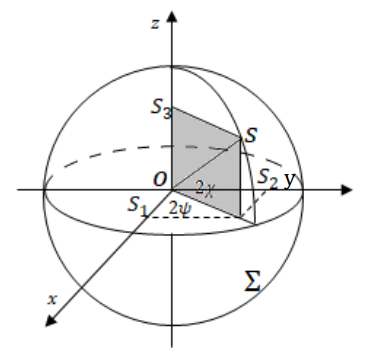
\includegraphics[width=0.35\textwidth]{img//14.png}
	\caption{庞加莱球示意图}
	\label{fig:14}
\end{figure}

偏振椭圆和斯托克斯参数的换算方法如下图:$S_0$表示椭圆的整体大小,$S_1$和$S_2$表
示椭圆在观测平面内的相对方向,$S_3$表示椭圆偏振的旋转方向。

\begin{figure}[H]
	\centering
	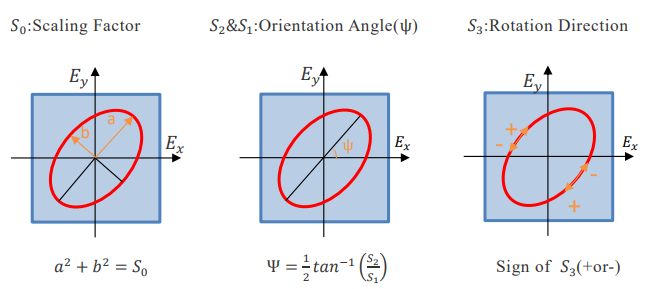
\includegraphics[width=\textwidth]{img//15.png}
	\caption{偏振椭圆}
	\label{fig:15}
\end{figure}

为减少实验误差,往往会采取尽可能少的测量量,导出斯托
克斯参数测量的经典方法。首先在光路中插入线偏振片,然后分别记录透射轴为水平
($P_x$)、垂直($P_y$)和$+45^{\circ}$时的功率,根据这三个功率值算出前三个斯托克斯参数。这三次测量都不用 1/4 波
片。为了得到第四个斯托克斯参数,我们要在$+45^{\circ}$线偏振片前面插入快轴沿水平方向
的 1/4 波片,测量功率($P_R$)后就能算出第四个斯托克斯参数。
\[\left\{
\begin{aligned}
&S_0=P_x+P_y\\
&S_1=P_x-P_y\\
&S_2=2P_{+45}-S_0\\
&S_3=S_0-2P_R\\
\end{aligned}
\right.
\]

• $S_0$表示总光强,它通常用单位 1 表示,其它三个数值相应地归一化。

• $S_1$表示水平偏振光强与垂直偏振光强之差,$S_1 \in [-1,1]$ ,数值为+1 说明全是水平偏振
光,-1 则全是垂直偏振光。

• $S_2$表示+45°偏振光强与-45°偏振光强之差,$S_2 \in [-1,1]$,数值为+1 说明全是+45°偏
振光,-1 则全是-45°偏振光。

• $S_3$表示右旋圆偏振光强与左旋圆偏振光强之差,$S_3 \in [-1,1]$,数值为+1 说明全是右旋
圆偏振光,-1 则全是左旋圆偏振光。

定义 $S = (S_0 S_1 S_2 S_3)^{T}$

T为斯托克斯矢量,容易得出

\begin{figure}[H]
	\centering
	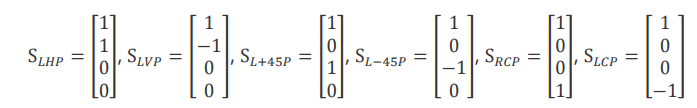
\includegraphics[width=0.8\textwidth]{img//16.png}
\end{figure}


标准单模光纤在实际使用中必然会偏离完美的圆对称,即使偏差非常小。这些偏
差主要可分以下三种:

几何偏差,比如纤芯不对称或偏离中心。

光学偏差,比如材料折射率不是均匀的。

力学偏差,由此导致应力双折射。

力学偏差的原因之一是光纤中存在张力。光纤在生产过程中迅速冷却,这本身就
容易引入张力,而光纤在使用中发生弯曲也会有张力。由于偏离完美的圆对称,两正
交偏振平面不再是任意选择的,而且两种偏振模式沿光纤传播时将出现时间差,由此
导致偏振模色散。

\section{实验仪器}
激光器、光纤耦合调节架、光纤 3 根(芯径分别为 4$\mu m$、9$\mu m$、62.5$\mu m$)、光纤耦合光功率
计、护目镜,SGQ-3 型光纤信息实验系统,包括了激光器、
调节架、观察屏和白屏等部件,偏振片,1/4$\lambda$@633nm 波片,光纤耦合调
整架,FC/PC 单模光纤

\section{实验结果}
\subsection{光纤光学}
\subsubsection{光纤耦合效率测量}
测量激光器输出光功率,重复五次,得输出光功率均值为:$P_0=2.304mW$
\\ \hspace*{\fill} \\

1. 直接耦合

单模光纤芯径为4$\mu m$,五次测量其直接耦合光功率均值为:$P_1=0.0718\mu W$

耦合效率为:
\begin{equation*}
	\eta_1=\frac{P_1}{P_0}=3.12\times10^{-3}\%
\end{equation*}

损耗为:
\begin{equation*}
	\gamma_1=-10log\left(\frac{P_1}{P_0}\right)=45.06dB
\end{equation*}

对于芯径为9$\mu m$的单模光纤重复同样操作,得直接耦合光功率均值为:$P_2=0.1906\mu W$

耦合效率为:
\begin{equation*}
	\eta_2=\frac{P_2}{P_0}=8.27\times10^{-3}\%
\end{equation*}

损耗为:
\begin{equation*}
	\gamma_2=-10log\left(\frac{P_2}{P_0}\right)=40.82dB
\end{equation*}

相同的,当对芯径为62.5$\mu m$的多模光纤重复同样操作得直接耦合光功率均值为:$P_3=6.938\mu W$

耦合效率为:
\begin{equation*}
	\eta_3=\frac{P_3}{P_0}=0.30\%
\end{equation*}

损耗为:
\begin{equation*}
	\gamma_3=-10log\left(\frac{P_3}{P_0}\right)=25.21dB
\end{equation*}
\\ \hspace*{\fill} \\

2. 透镜耦合

芯径为4$\mu m$的单模光纤,五次测量其透镜耦合光功率均值为:$P_1=1.0472 m W$

耦合效率为:
\begin{equation*}
	\eta_1=\frac{P_1}{P_0}=45.45\%
\end{equation*}

损耗为:
\begin{equation*}
	\gamma_1=-10log\left(\frac{P_1}{P_0}\right)=3.42dB
\end{equation*}

对于芯径为9$\mu m$的单模光纤重复同样操作,得直接耦合光功率均值为:$P_2=1.644m W$

耦合效率为:
\begin{equation*}
	\eta_2=\frac{P_2}{P_0}=71.35\%
\end{equation*}

损耗为:
\begin{equation*}
	\gamma_2=-10log\left(\frac{P_2}{P_0}\right)=1.46dB
\end{equation*}

相同的,当对芯径为62.5$\mu m$的多模光纤重复同样操作得直接耦合光功率均值为:$P_3=1.70 mW$

耦合效率为:
\begin{equation*}
	\eta_3=\frac{P_3}{P_0}=73.78\%
\end{equation*}

损耗为:
\begin{equation*}
	\gamma_3=-10log\left(\frac{P_3}{P_0}\right)=1.32dB
\end{equation*}
\\ \hspace*{\fill} \\

从数据中我们可以看出,用同一种耦合方式耦合时,光纤直径越大,其耦合效率越高,传输损耗越低。
将直接耦合方法与透镜耦合方式比较,透镜耦合的效率显著高于直接耦合,并且传输损耗大大降低。这与透镜聚焦,将光功率汇集于焦点的功能息息相关。

\subsubsection{光纤数值孔径测量}

使用单模光纤, 调节至耦合效率最大, 测量白屏上光斑的直径 d 与光纤输出端面到白
屏距离 L 的关系, 记录数据如表\ref{tab:NA4}和表\ref{tab:NA9},其中数值孔径计算式为:
\begin{equation*}
	NA=\frac{d}{\sqrt{4L^2+d^2}}
\end{equation*}
\begin{table}[H]
	\caption{$4\mu m$ 光纤数值孔径}
	\centering
	  \begin{tabular}{lrrrrrrrr}
		\toprule
	  距离L(cm) & 4.5   & 5.5   & 6.5   & 7.5   & 8.5   & 9.5   & 10.5  & 11.5 \\
	  直径d(cm) & 1.61  & 2.02  & 2.35  & 2.72  & 3.16  & 3.49  & 3.94  & 4.41 \\
	  数值孔径NA & 0.17609 & 0.180616 & 0.177886 & 0.178424 & 0.182752 & 0.180662 & 0.184402 & 0.188309 \\
	    \bottomrule
	  \end{tabular}%
	\label{tab:NA4}%
  \end{table}%

  数值孔径平均值:
  \begin{equation*}
	  \overline{NA}=0.181143 
  \end{equation*}

  平均值的试验标准差:
  \begin{equation*}
	  \eta = \sqrt{\frac{1}{8\times7} \sum_{i = 1}^{8} \left(NA_i-\overline{NA}\right)^2 }=0.003938
  \end{equation*}

  故$4\mu m$芯径的光纤数值孔径为:$NA=0.181143\pm0.003938$
  
\begin{table}[H]
	\caption{$9\mu m$ 光纤数值孔径}
	\centering
	  \begin{tabular}{lrrrrrrrr}
		\toprule
	  距离L(cm) & 4.5   & 5.5   & 6.5   & 7.5   & 8.5   & 9.5   & 10.5  & 11.5 \\
	  直径d(cm) & 1.53  & 1.92  & 2.23  & 2.70  & 3.13  & 3.69  & 4.08  & 4.51 \\
	  数值孔径NA & 0.1676 & 0.171946 & 0.169069 & 0.177153 & 0.181074 & 0.190648 & 0.19072 & 0.192423 \\
    	\bottomrule
	  \end{tabular}%
	\label{tab:NA9}%
  \end{table}%

  数值孔径平均值:
  \begin{equation*}
	  \overline{NA}=0.180078 
  \end{equation*}

  平均值的试验标准差:
  \begin{equation*}
	  \eta = \sqrt{\frac{1}{8\times7} \sum_{i = 1}^{8} \left(NA_i-\overline{NA}\right)^2 }=0.010212
  \end{equation*}

  故$9\mu m$芯径的光纤数值孔径为:$NA=0.180078\pm0.010212$


使用多模光纤, 调节至耦合效率最大, 测量白屏上光斑的直径 d 与光纤输出端面到白
屏距离 L 的关系, 记录数据如表\ref{tab:NA62.5}: 
  
\begin{table}[H]
	\caption{$62.5\mu m$ 光纤数值孔径}
	\centering
	  \begin{tabular}{lrrrrrrrr}
		\toprule
	  距离L(cm) & 4.5   & 5.5   & 6.5   & 7.5   & 8.5   & 9.5   & 10.5  & 11.5 \\
	  直径d(cm) & 2.61  & 3.20   & 3.82  & 4.25  & 4.71  & 5.42  & 6.03  & 6.78 \\
	  数值孔径NA & 0.27852 & 0.27933 & 0.281927 & 0.272603 & 0.267001 & 0.27432 & 0.27599 & 0.282753 \\
	    \bottomrule
	  \end{tabular}%
	\label{tab:NA62.5}%
  \end{table}%

  数值孔径平均值:
  \begin{equation*}
	  \overline{NA}=0.276556 
  \end{equation*}

  平均值的试验标准差:
  \begin{equation*}
	  \eta = \sqrt{\frac{1}{8\times7} \sum_{i = 1}^{8} \left(NA_i-\overline{NA}\right)^2 }=0.005225
  \end{equation*}

  故$62.5\mu m$芯径的光纤数值孔径为:$NA=0.0.276556\pm0.005225$


\begin{figure}[H]
	\centering
	\subfloat[芯径$4\mu m$光纤光斑]
	{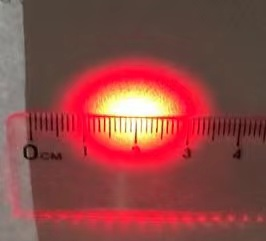
\includegraphics[width=0.27\textwidth]{img//sp4.jpg}
	}%
	\subfloat[芯径$9\mu m$光纤光斑]
	{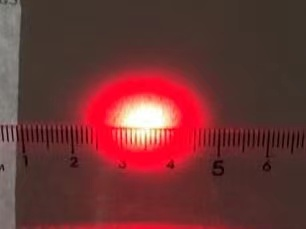
\includegraphics[width=0.31\textwidth]{img//sp9.jpg}
	}%
	\subfloat[芯径$62.5\mu m$光纤光斑]
	{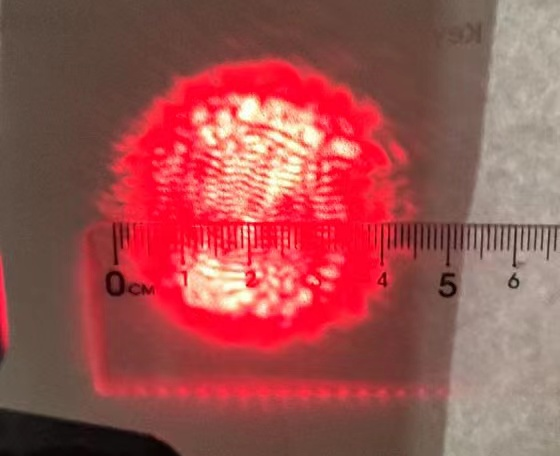
\includegraphics[width=0.29\textwidth]{img//sp625.jpg}
	}%
	\caption{不同芯径光纤距输出端7.5cm所得光斑}
	\label{fig:sp}
\end{figure}


\subsection{光纤传感器}
\subsubsection{光纤压力传感器}

转动光纤干涉仪上的测微螺杆,观察显示屏上条纹的移动。读取条纹移动数及螺杆读数,记录如表\ref{tab:P}:

\begin{table}[htbp]
	\centering
	\caption{条纹数目随螺杆刻度改变}
	  \begin{tabular}{rrrrr}
	  \multicolumn{1}{l}{条纹移动数n} & \multicolumn{1}{l}{螺杆刻度mm} & \multicolumn{1}{l}{螺杆刻度mm} & \multicolumn{1}{l}{螺杆刻度mm} & \multicolumn{1}{l}{螺杆刻度mm} \\
	  0     & 0.05  & 2.628 & 0.15  & 2.335 \\
	  1     & 0.211 & 2.47  & 0.27  & 2.179 \\
	  2     & 0.366 & 2.298 & 0.452 & 2.03 \\
	  3     & 0.567 & 2.101 & 0.55  & 1.85 \\
	  4     & 0.742 & 1.968 & 0.73  & 1.704 \\
	  5     & 0.919 & 1.808 & 0.835 & 1.535 \\
	  6     & 1.038 & 1.649 & 1.02  & 1.406 \\
	  7     & 1.273 & 1.464 & 1.151 & 1.253 \\
	  8     & 1.442 & 1.321 & 1.281 & 1.112 \\
	  9     & 1.551 & 1.14  & 1.455 & 0.93 \\
	  10    & 1.75  & 1.004 & 1.585 & 0.778 \\
	  11    & 1.967 & 0.851 & 1.751 & 0.643 \\
	  12    & 2.104 & 0.77  & 1.919 & 0.472 \\
	  13    & 2.282 & 0.531 & 2.041 & 0.343 \\
	  14    & 2.472 & 0.369 & 2.189 & 0.135 \\
	  15    & 2.688 & 0.215 & 2.355 & 0.03 \\
	  \end{tabular}%
	\label{tab:P}%
  \end{table}%  

从左到右四列螺杆刻度分别为A组实验上行和下行读数,B组实验上行和下行读数。
将表\ref{tab:P}中的四组数据分别作折线图并且进行线性拟合,结果见图\ref{fig:P},拟合所得斜率分别为5.74253,-6.26419,6.78522,-6.48045.


\begin{figure}[htbp]
	\centering
	\subfloat[A组上行]{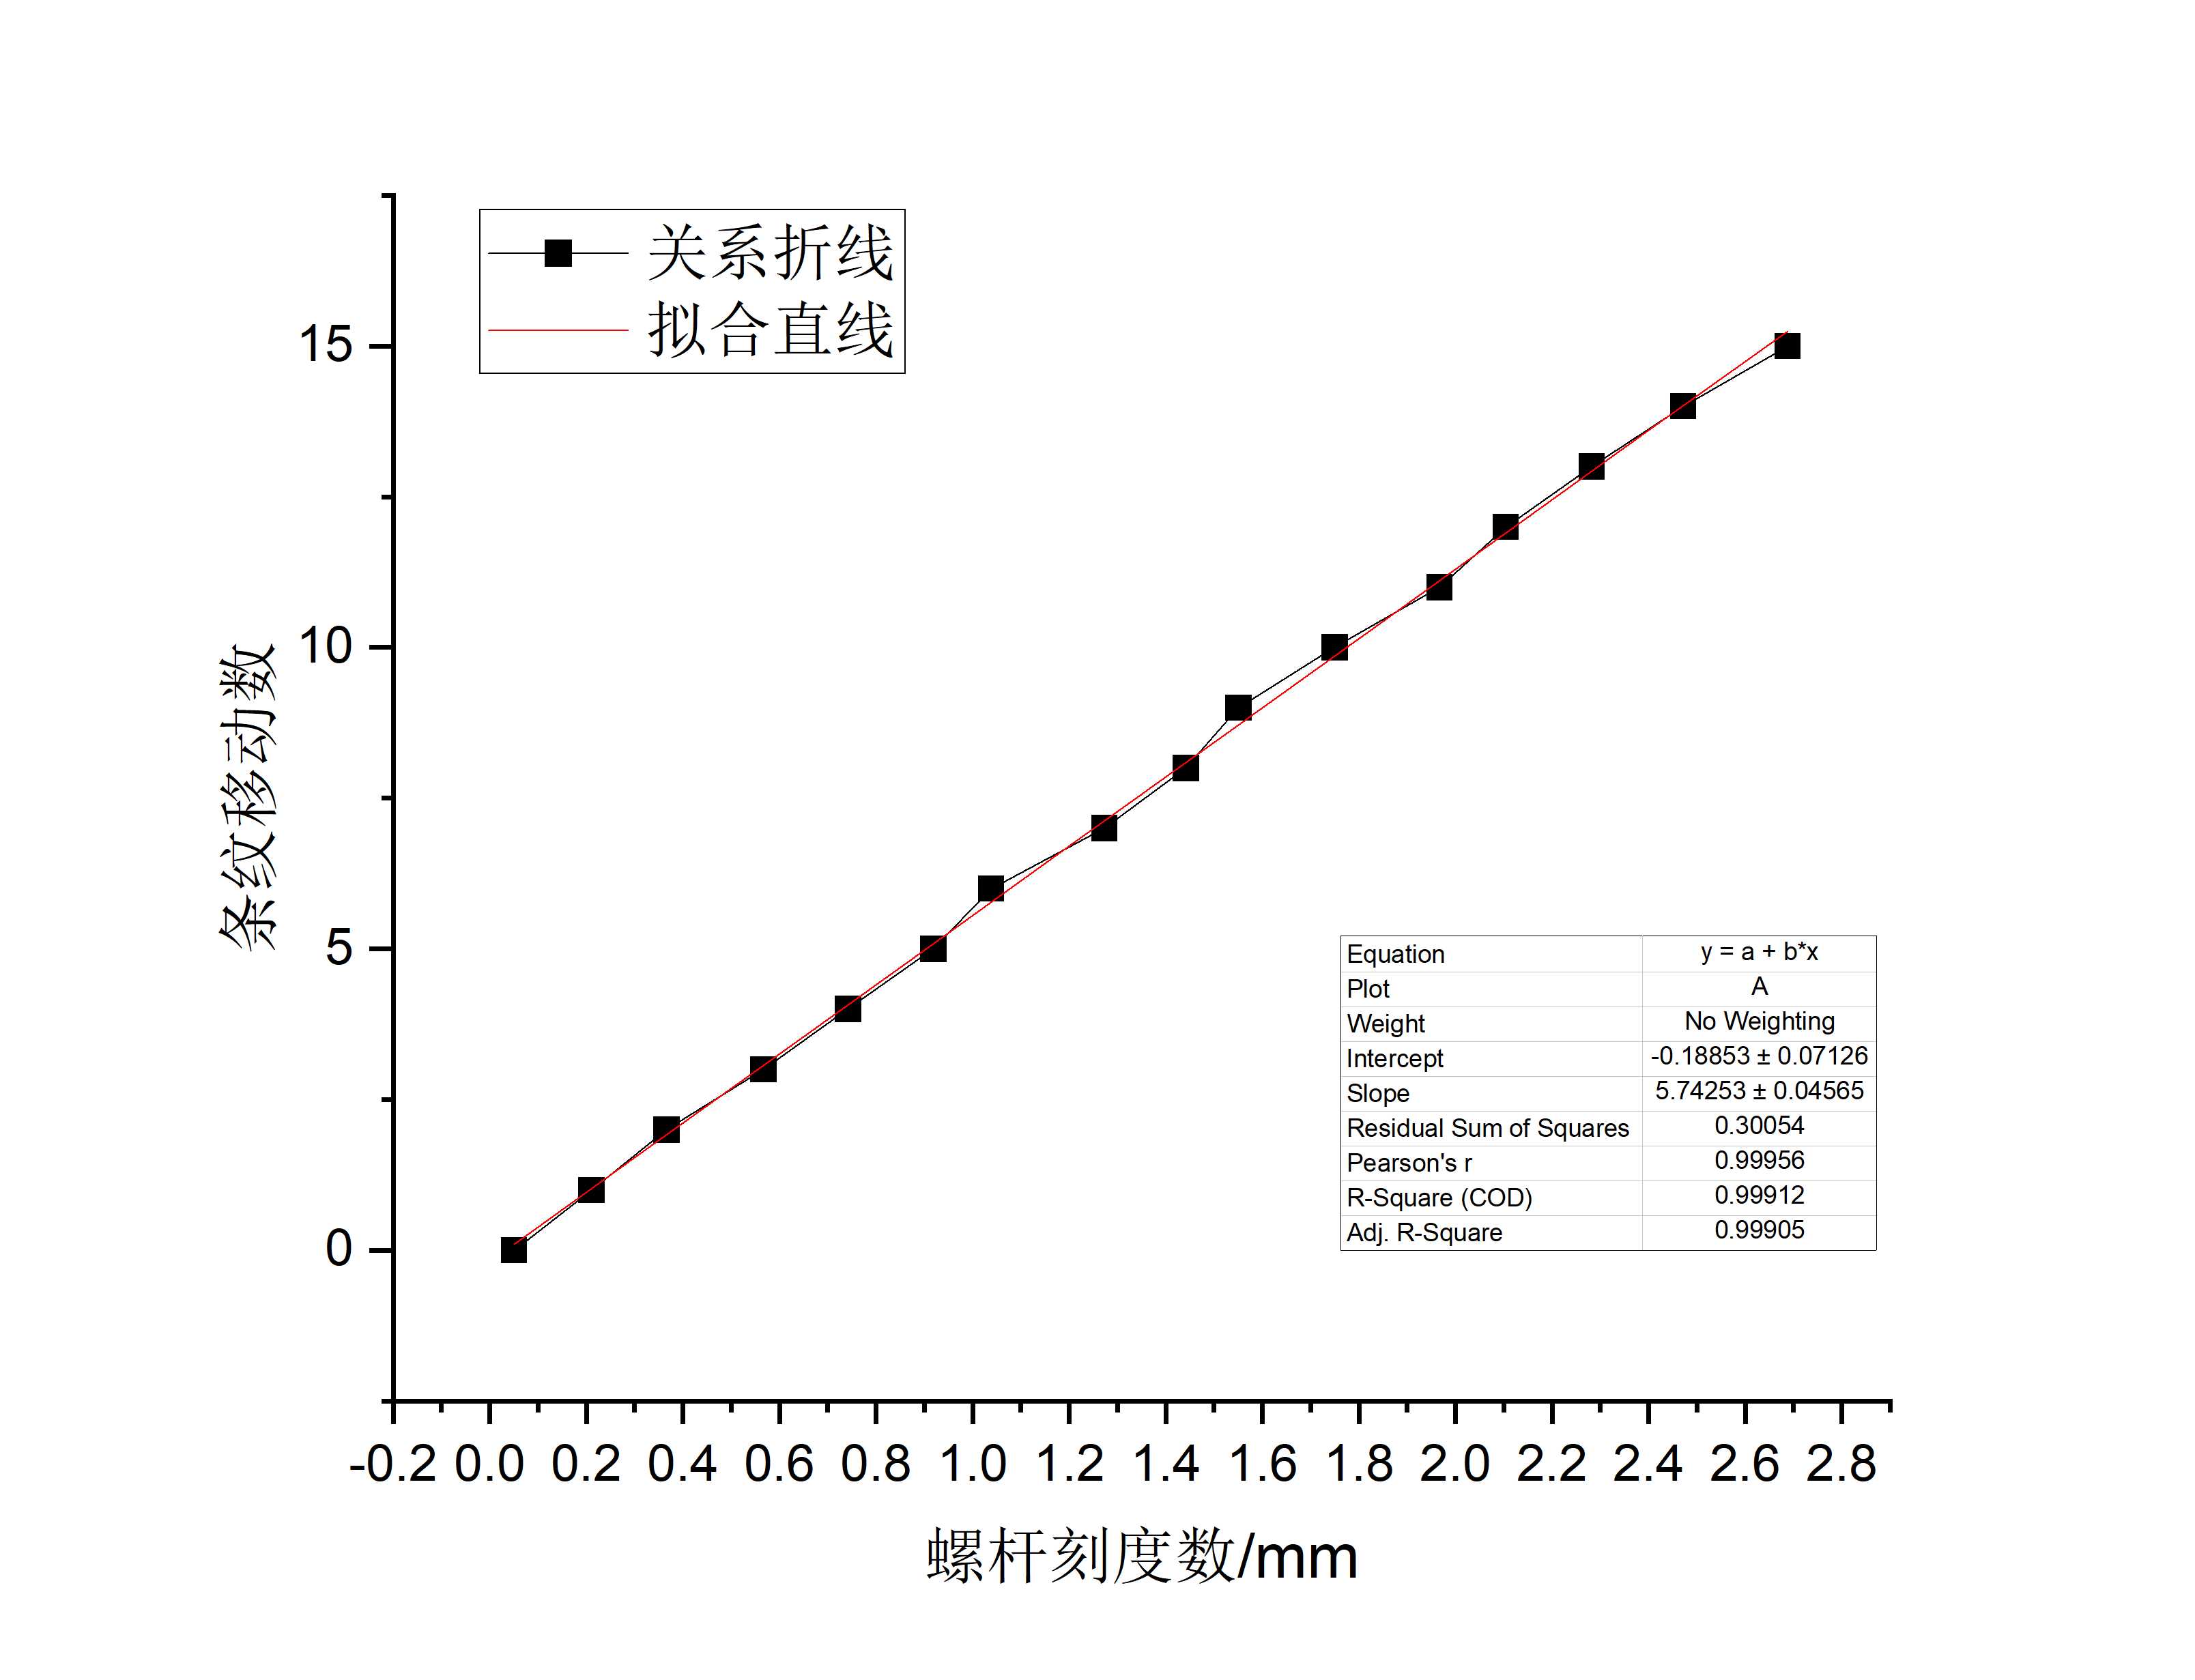
\includegraphics[width=0.48\textwidth]{img//PA1.png}}
	\subfloat[A组下行]{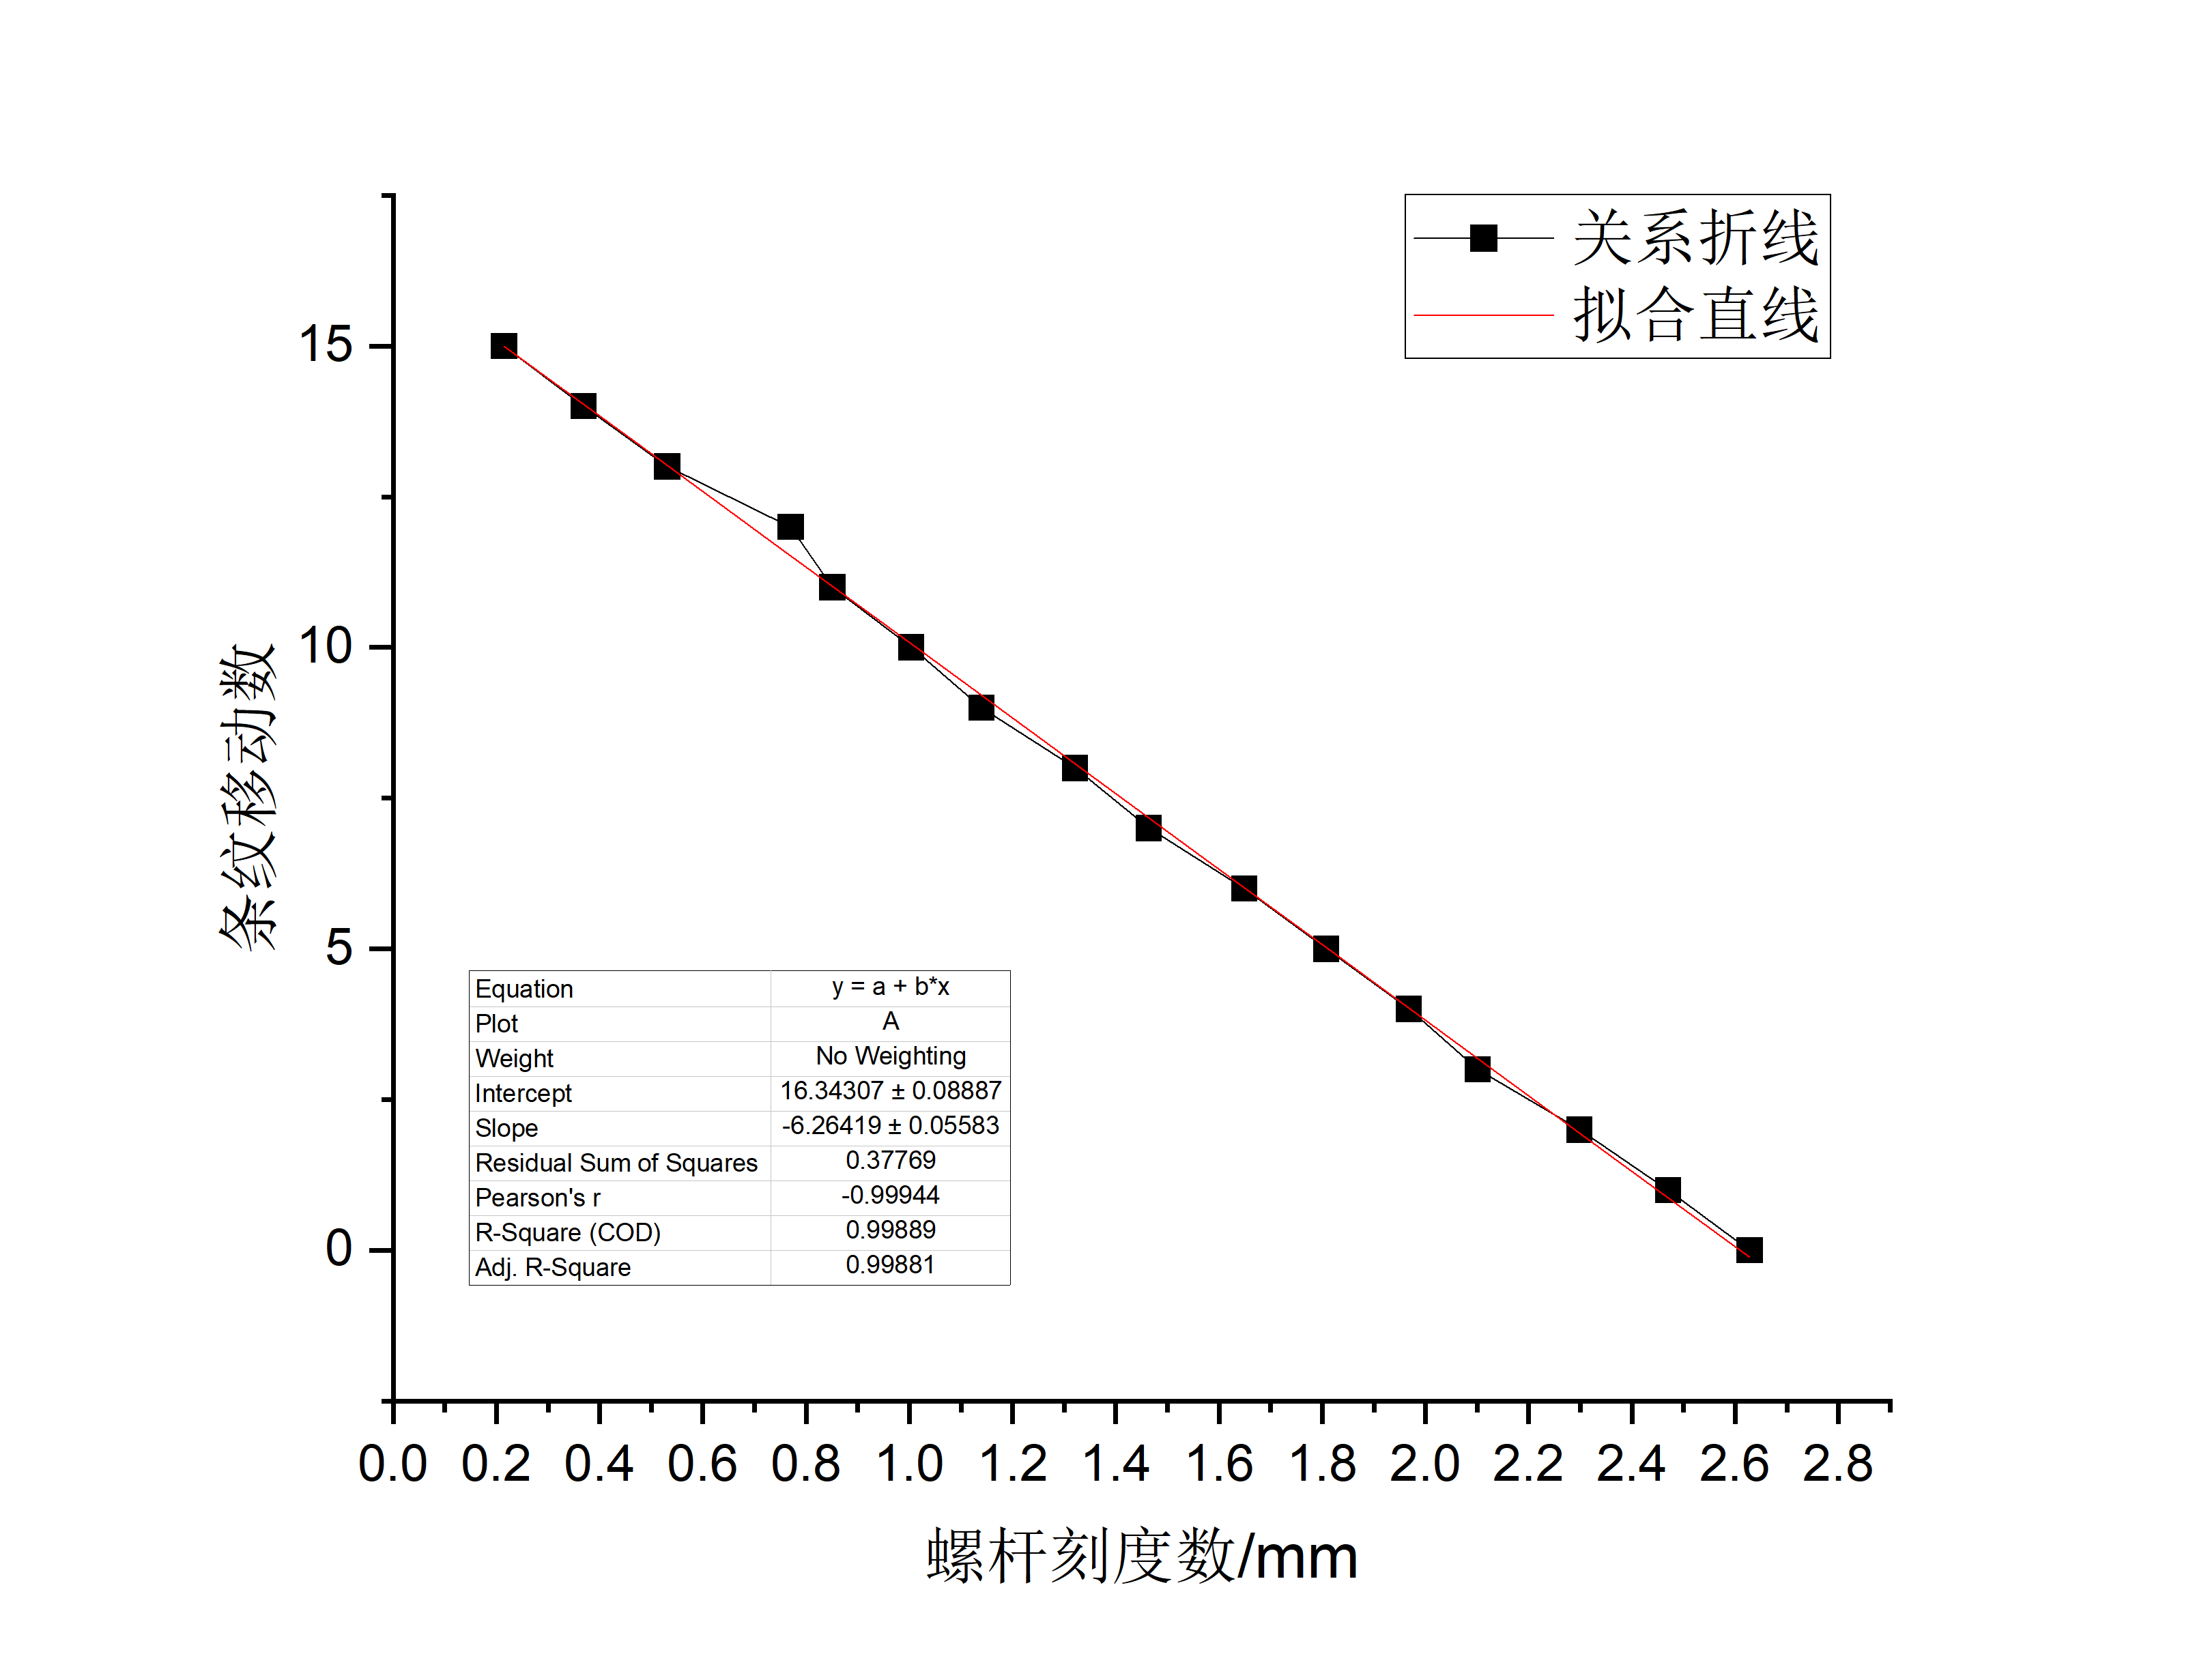
\includegraphics[width=0.48\textwidth]{img//PA2.png}}

	\subfloat[B组上行]{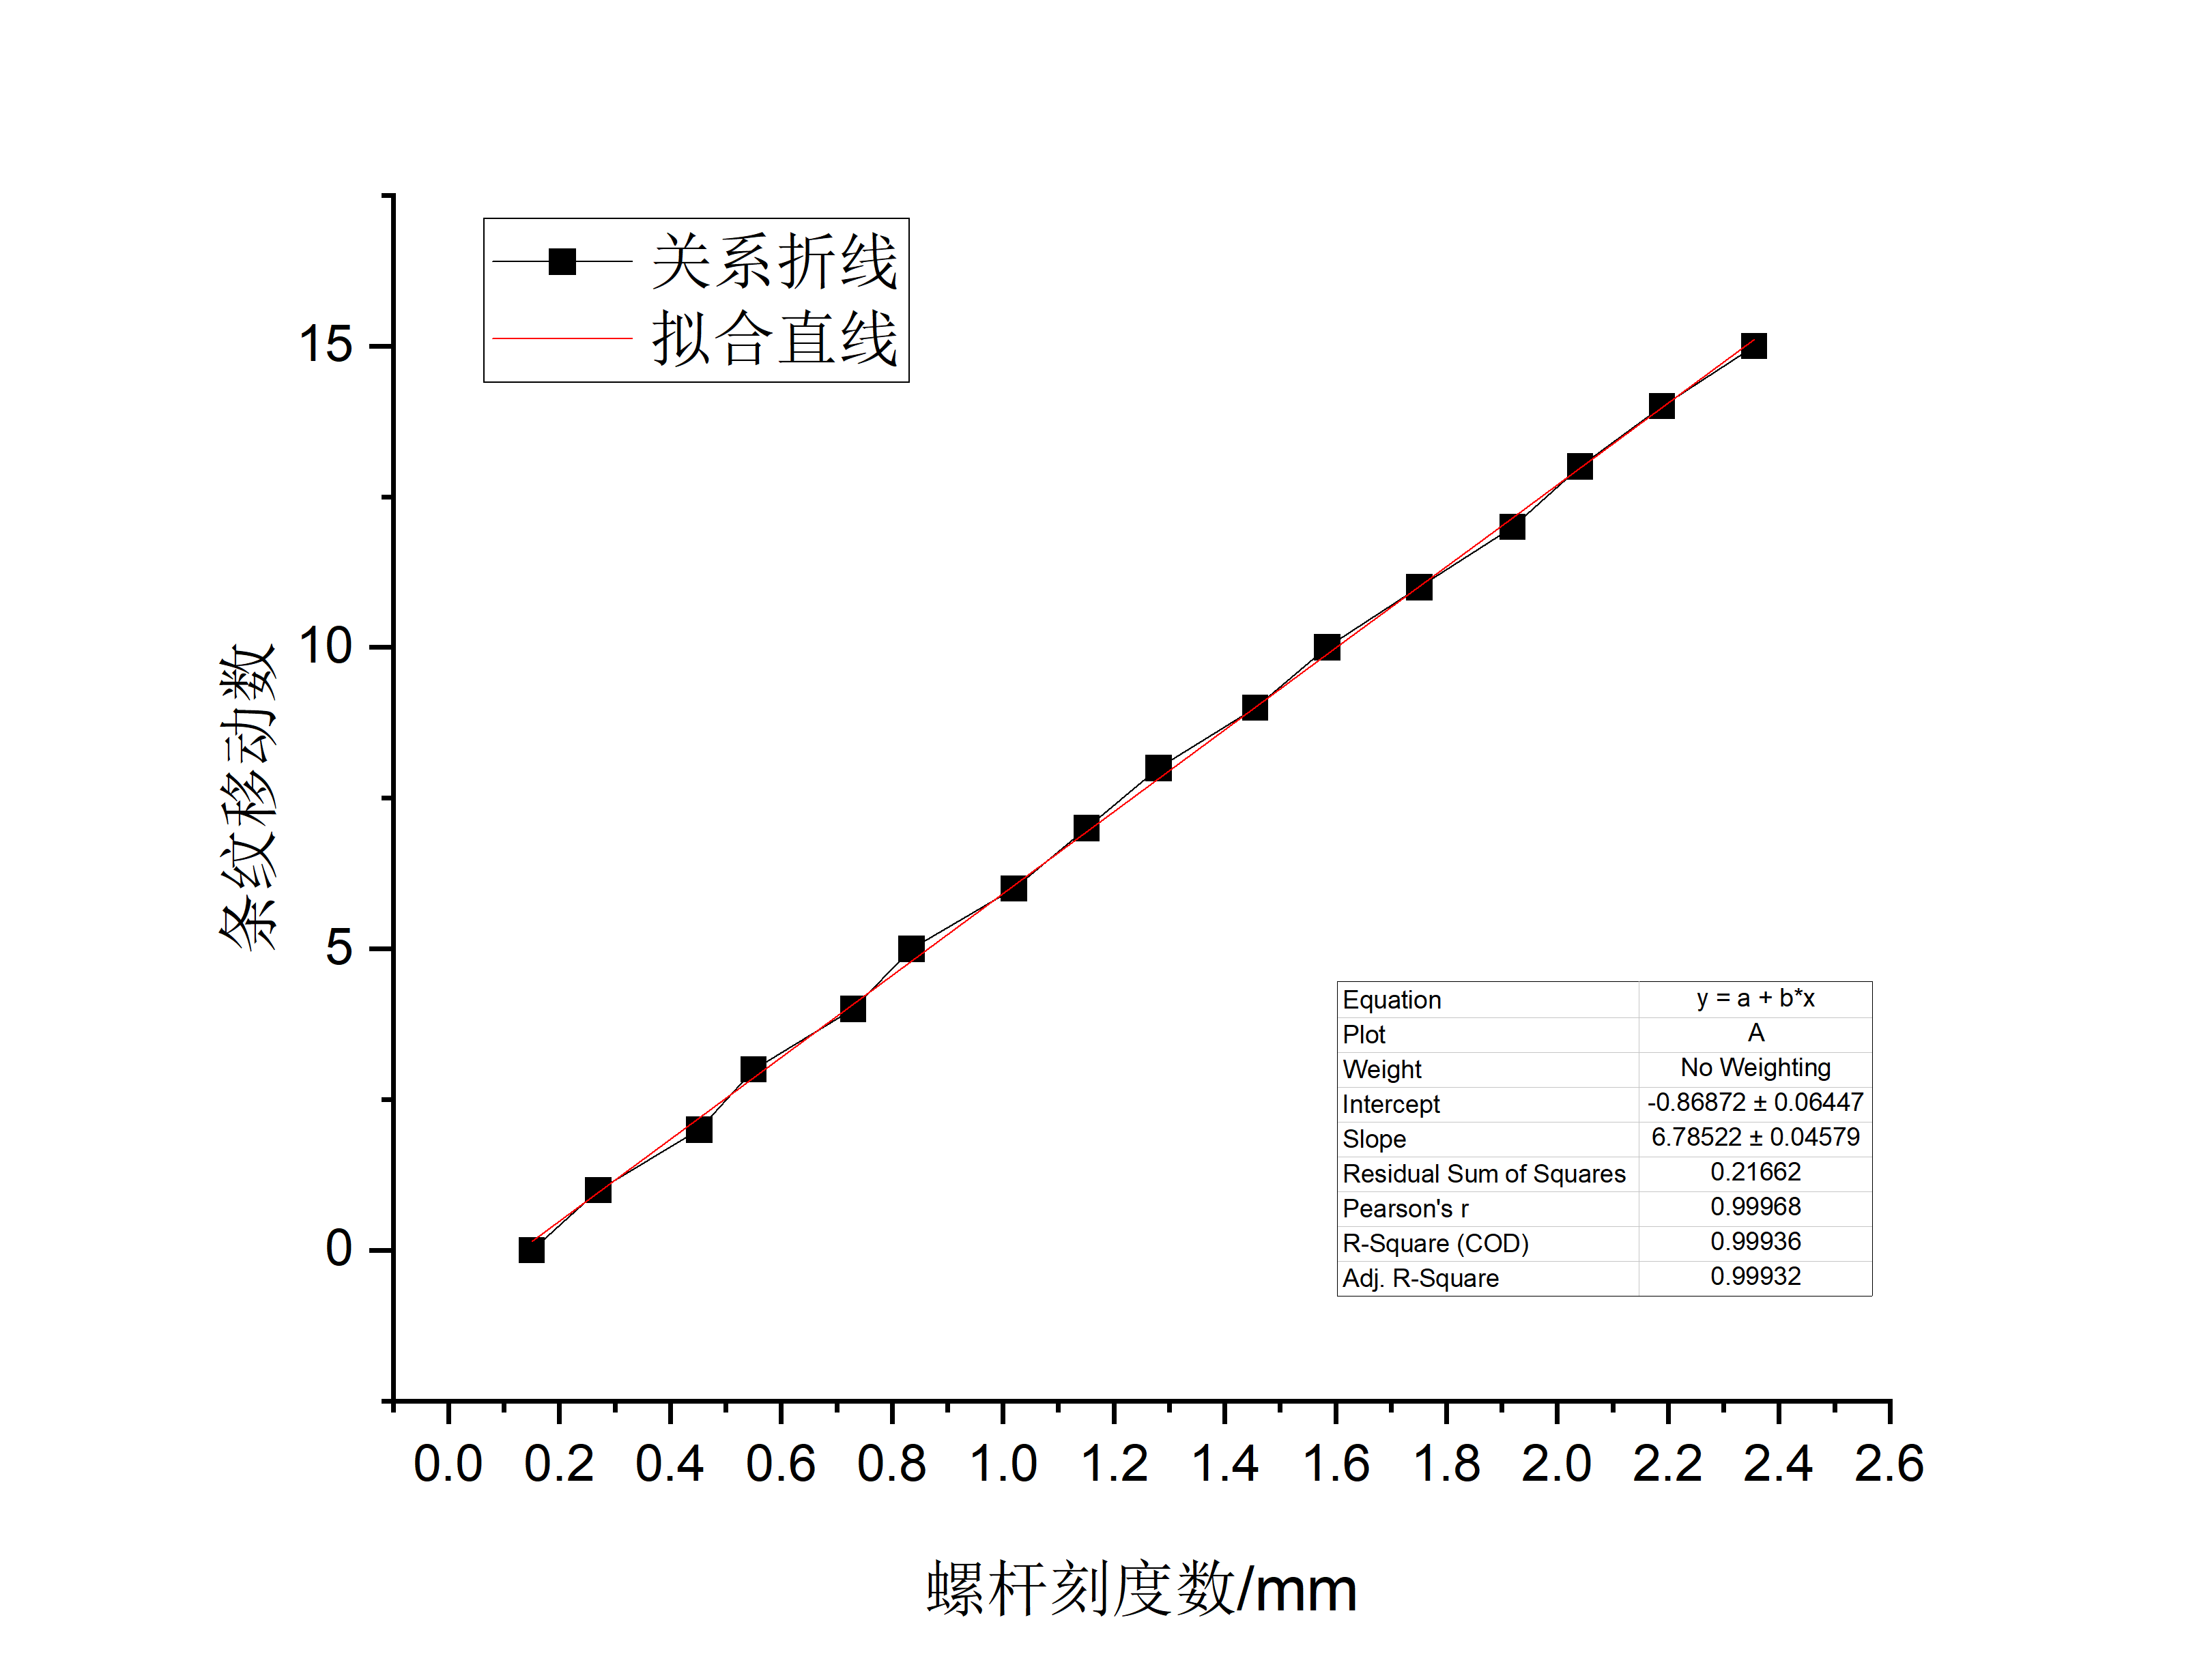
\includegraphics[width=0.48\textwidth]{img//PB1.png}}
	\subfloat[B组下行]{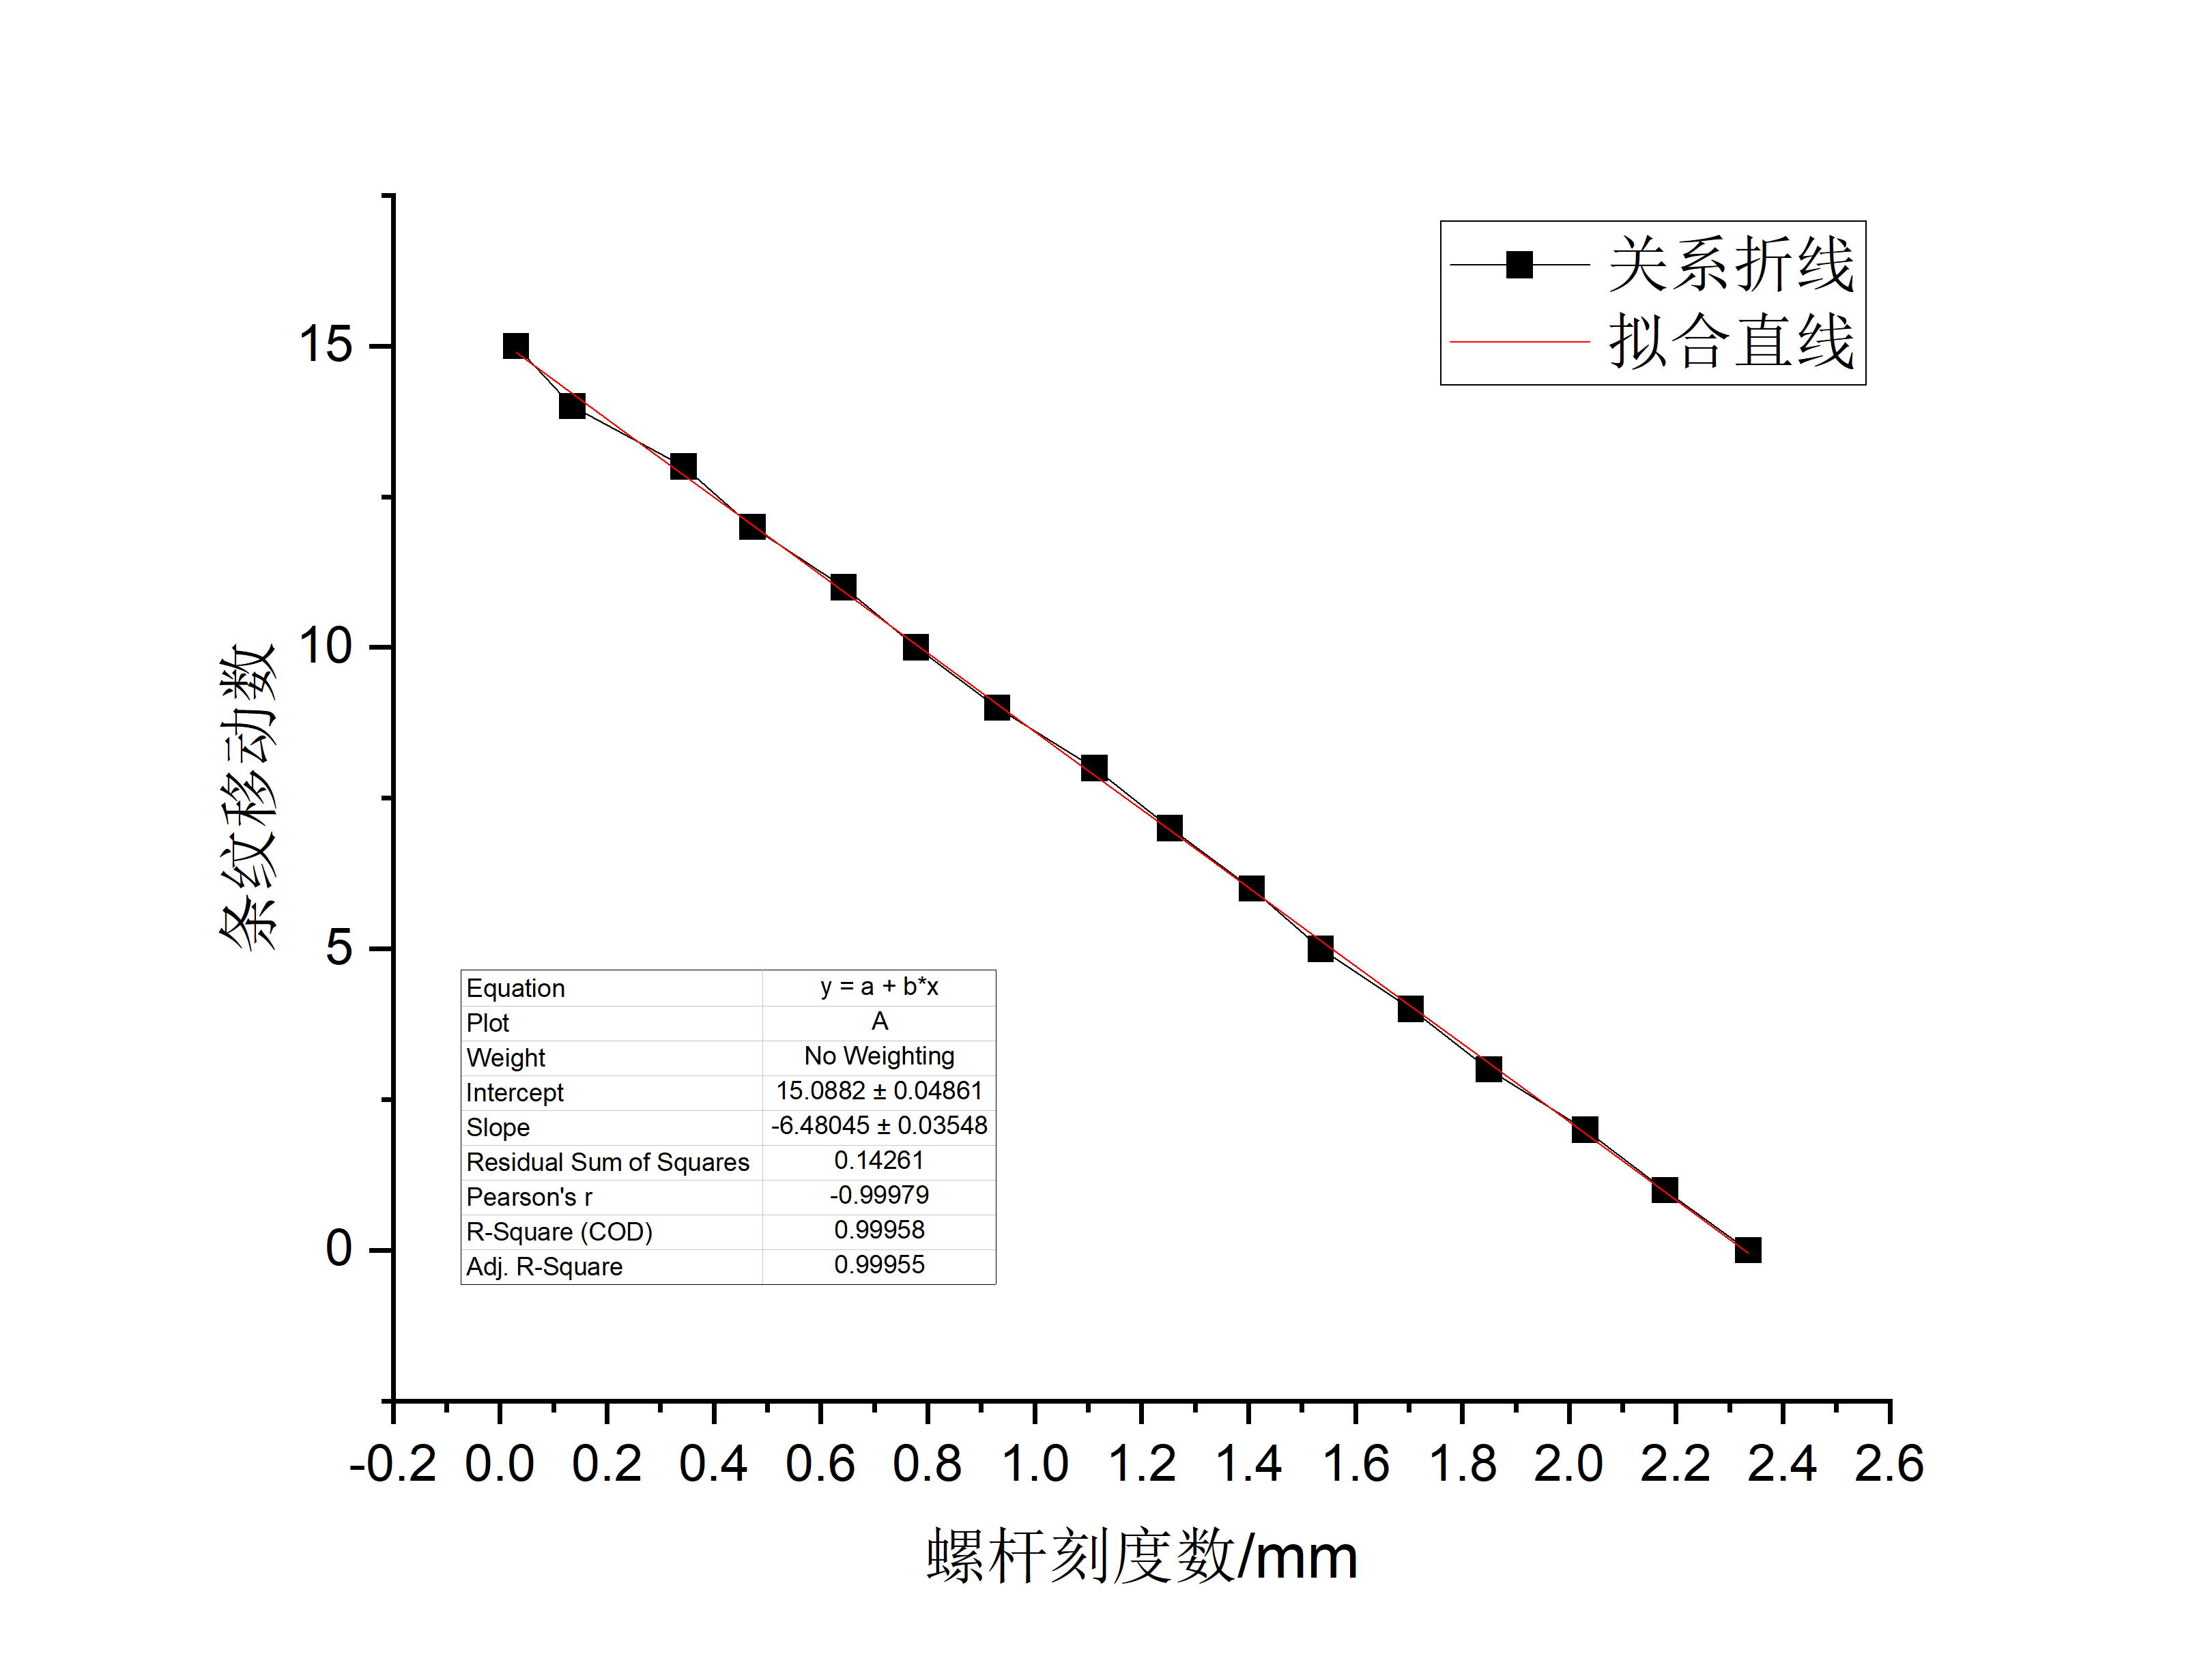
\includegraphics[width=0.48\textwidth]{img//PB2.png}}
	\caption{光纤压力传感器条纹移动数目随螺杆刻度变化关系}
	\label{fig:P}
\end{figure}

观察实验点的分布可知, 条纹移动数与螺旋刻度基本上呈线性关系, 进行线性拟合得到直线
相关系数均超过0.99,线性关系成立。 计算得斜率绝对值均值 $\overline{|K|}=6.32 $可知 对于该光纤压力传感器, 螺旋
刻度每增加 1mm, 条纹就会移动 6.32 条, 对应的光相位变化$\varDelta \phi=2\pi \varDelta n=39.70rad$ ,
所以, 每改变螺旋距离 1mm, 光纤传感器输出光的相位就会变化 39.70rad。

  
\subsubsection{光纤温度传感器}

由室温升至35摄氏度,观察显示屏上条纹的移动。读取条纹移动数及温度,记录如表\ref{tab:T}:

\begin{table}[htbp]
	\centering
	\caption{条纹数目随温度改变}
	  \begin{tabular}{rrrrr}
	  \multicolumn{1}{l}{条纹移动数n} & \multicolumn{1}{l}{温度($C^{\circ}$)} & \multicolumn{1}{l}{温度($C^{\circ}$)} & \multicolumn{1}{l}{温度($C^{\circ}$)} & \multicolumn{1}{l}{温度($C^{\circ}$)} \\
	  0     & 25.0    & 35.0    & 25.0    & 35.0 \\
	  5     & 25.5  & 34.5  & 25.5  & 34.6 \\
	  10    & 25.9  & 34.1  & 26.0    & 34.0 \\
	  15    & 26.5  & 33.6  & 26.6  & 33.5 \\
	  20    & 27.0    & 33.1  & 27.1  & 33.0 \\
	  25    & 27.4  & 32.6  & 27.5  & 32.6 \\
	  30    & 28.0    & 32.2  & 28.1  & 32.0 \\
	  35    & 28.6  & 31.5  & 28.6  & 31.5 \\
	  40    & 29.0    & 31.0    & 29.1  & 31.0 \\
	  45    & 29.5  & 30.4  & 29.5  & 30.4 \\
	  50    & 30.1  & 30.0    & 30.1  & 30.0 \\
	  55    & 30.6  & 29.6  & 30.5  & 29.6 \\
	  60    & 31.1  & 29.0    & 31.1  & 29.0 \\
	  65    & 31.6  & 28.5  & 31.5  & 28.5 \\
	  70    & 32.0    & 28.0    & 32.0    & 28.1 \\
	  75    & 32.4  & 27.6  & 32.5  & 27.5 \\
	  80    & 33.0    & 27.0    & 33.0    & 27.0 \\
	  85    & 33.5  & 26.4  & 33.4  & 26.6 \\
	  90    & 34.0    & 26.0    & 34.0     & 26.0 \\
	  95    & 34.4  & 25.5  & 34.5  & 25.6 \\
	  100   & 35.1  & 25.0    & 35.0    & 25.1 \\
	  \end{tabular}%
	\label{tab:T}%
  \end{table}%

从左到右四列温度分别为A组实验上行和下行读数,B组实验上行和下行读数。
将表\ref{tab:T}中的四组数据分别作折线图并且进行线性拟合,结果见图\ref{fig:T},拟合所得斜率分别为9.96398,-9.90802,10.06779,10.04388.

  \begin{figure}[htbp]
	\centering
	\subfloat[A组上行]{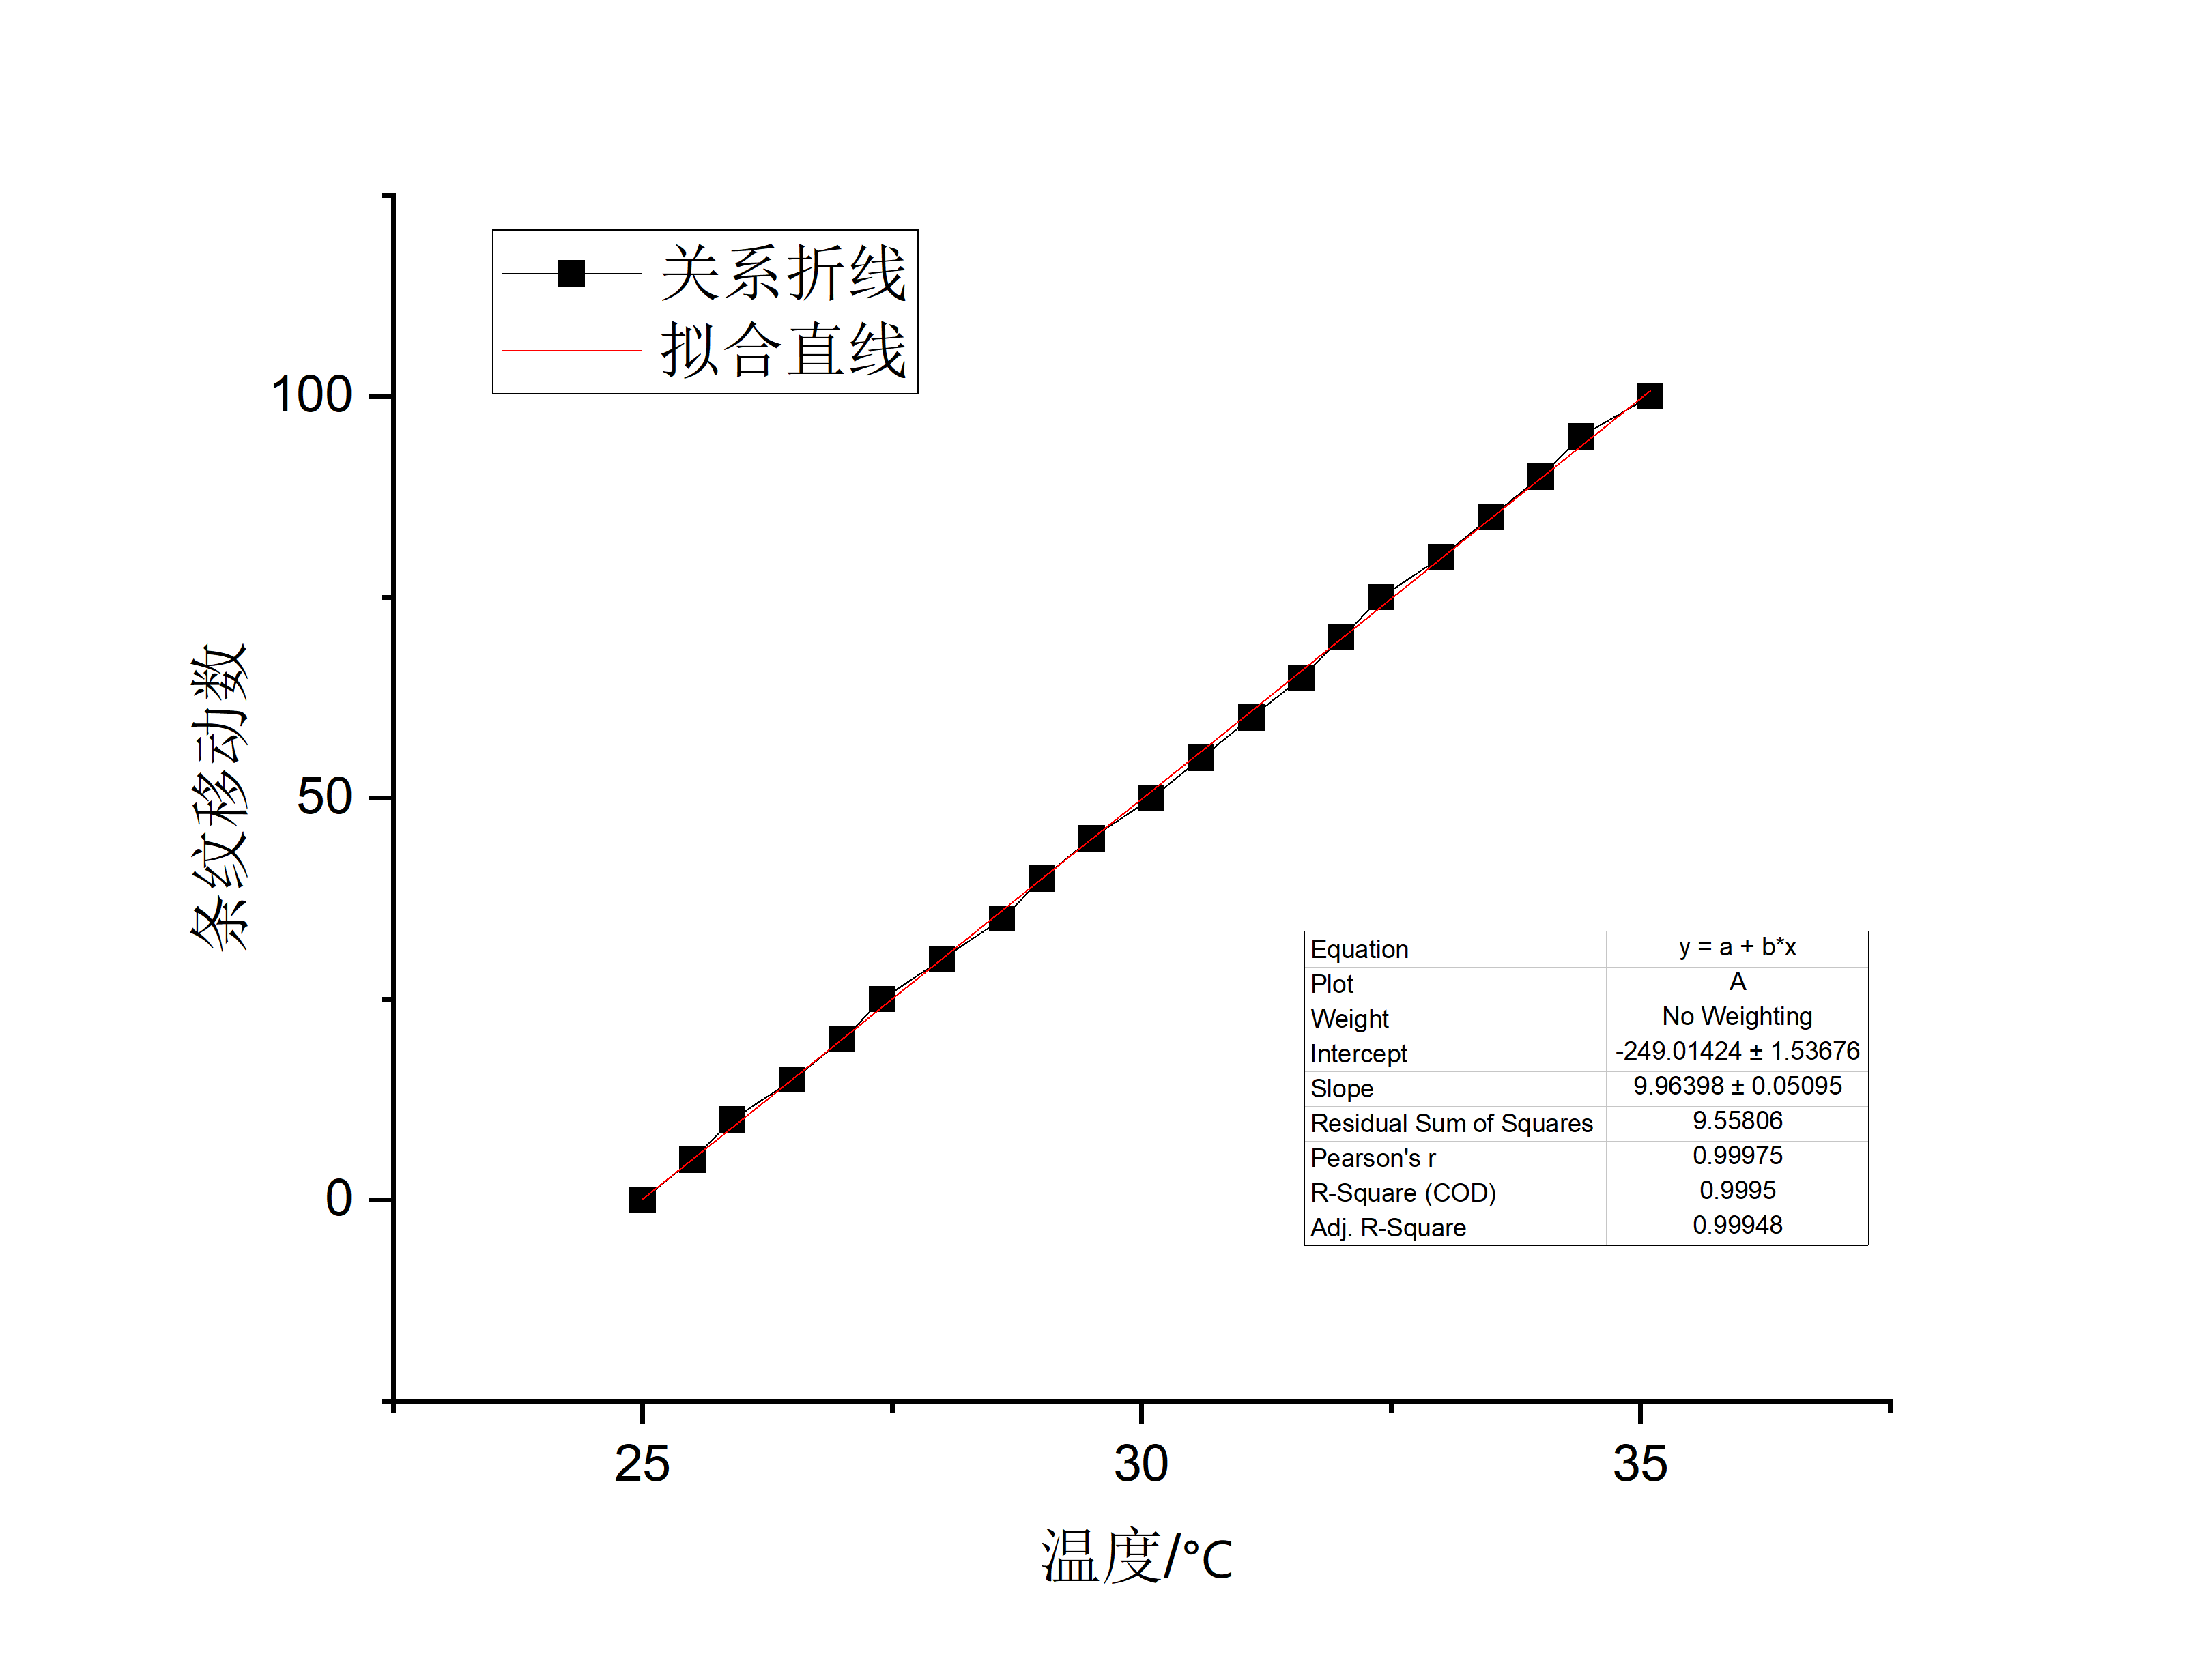
\includegraphics[width=0.48\textwidth]{img//TA1.png}}
	\subfloat[A组下行]{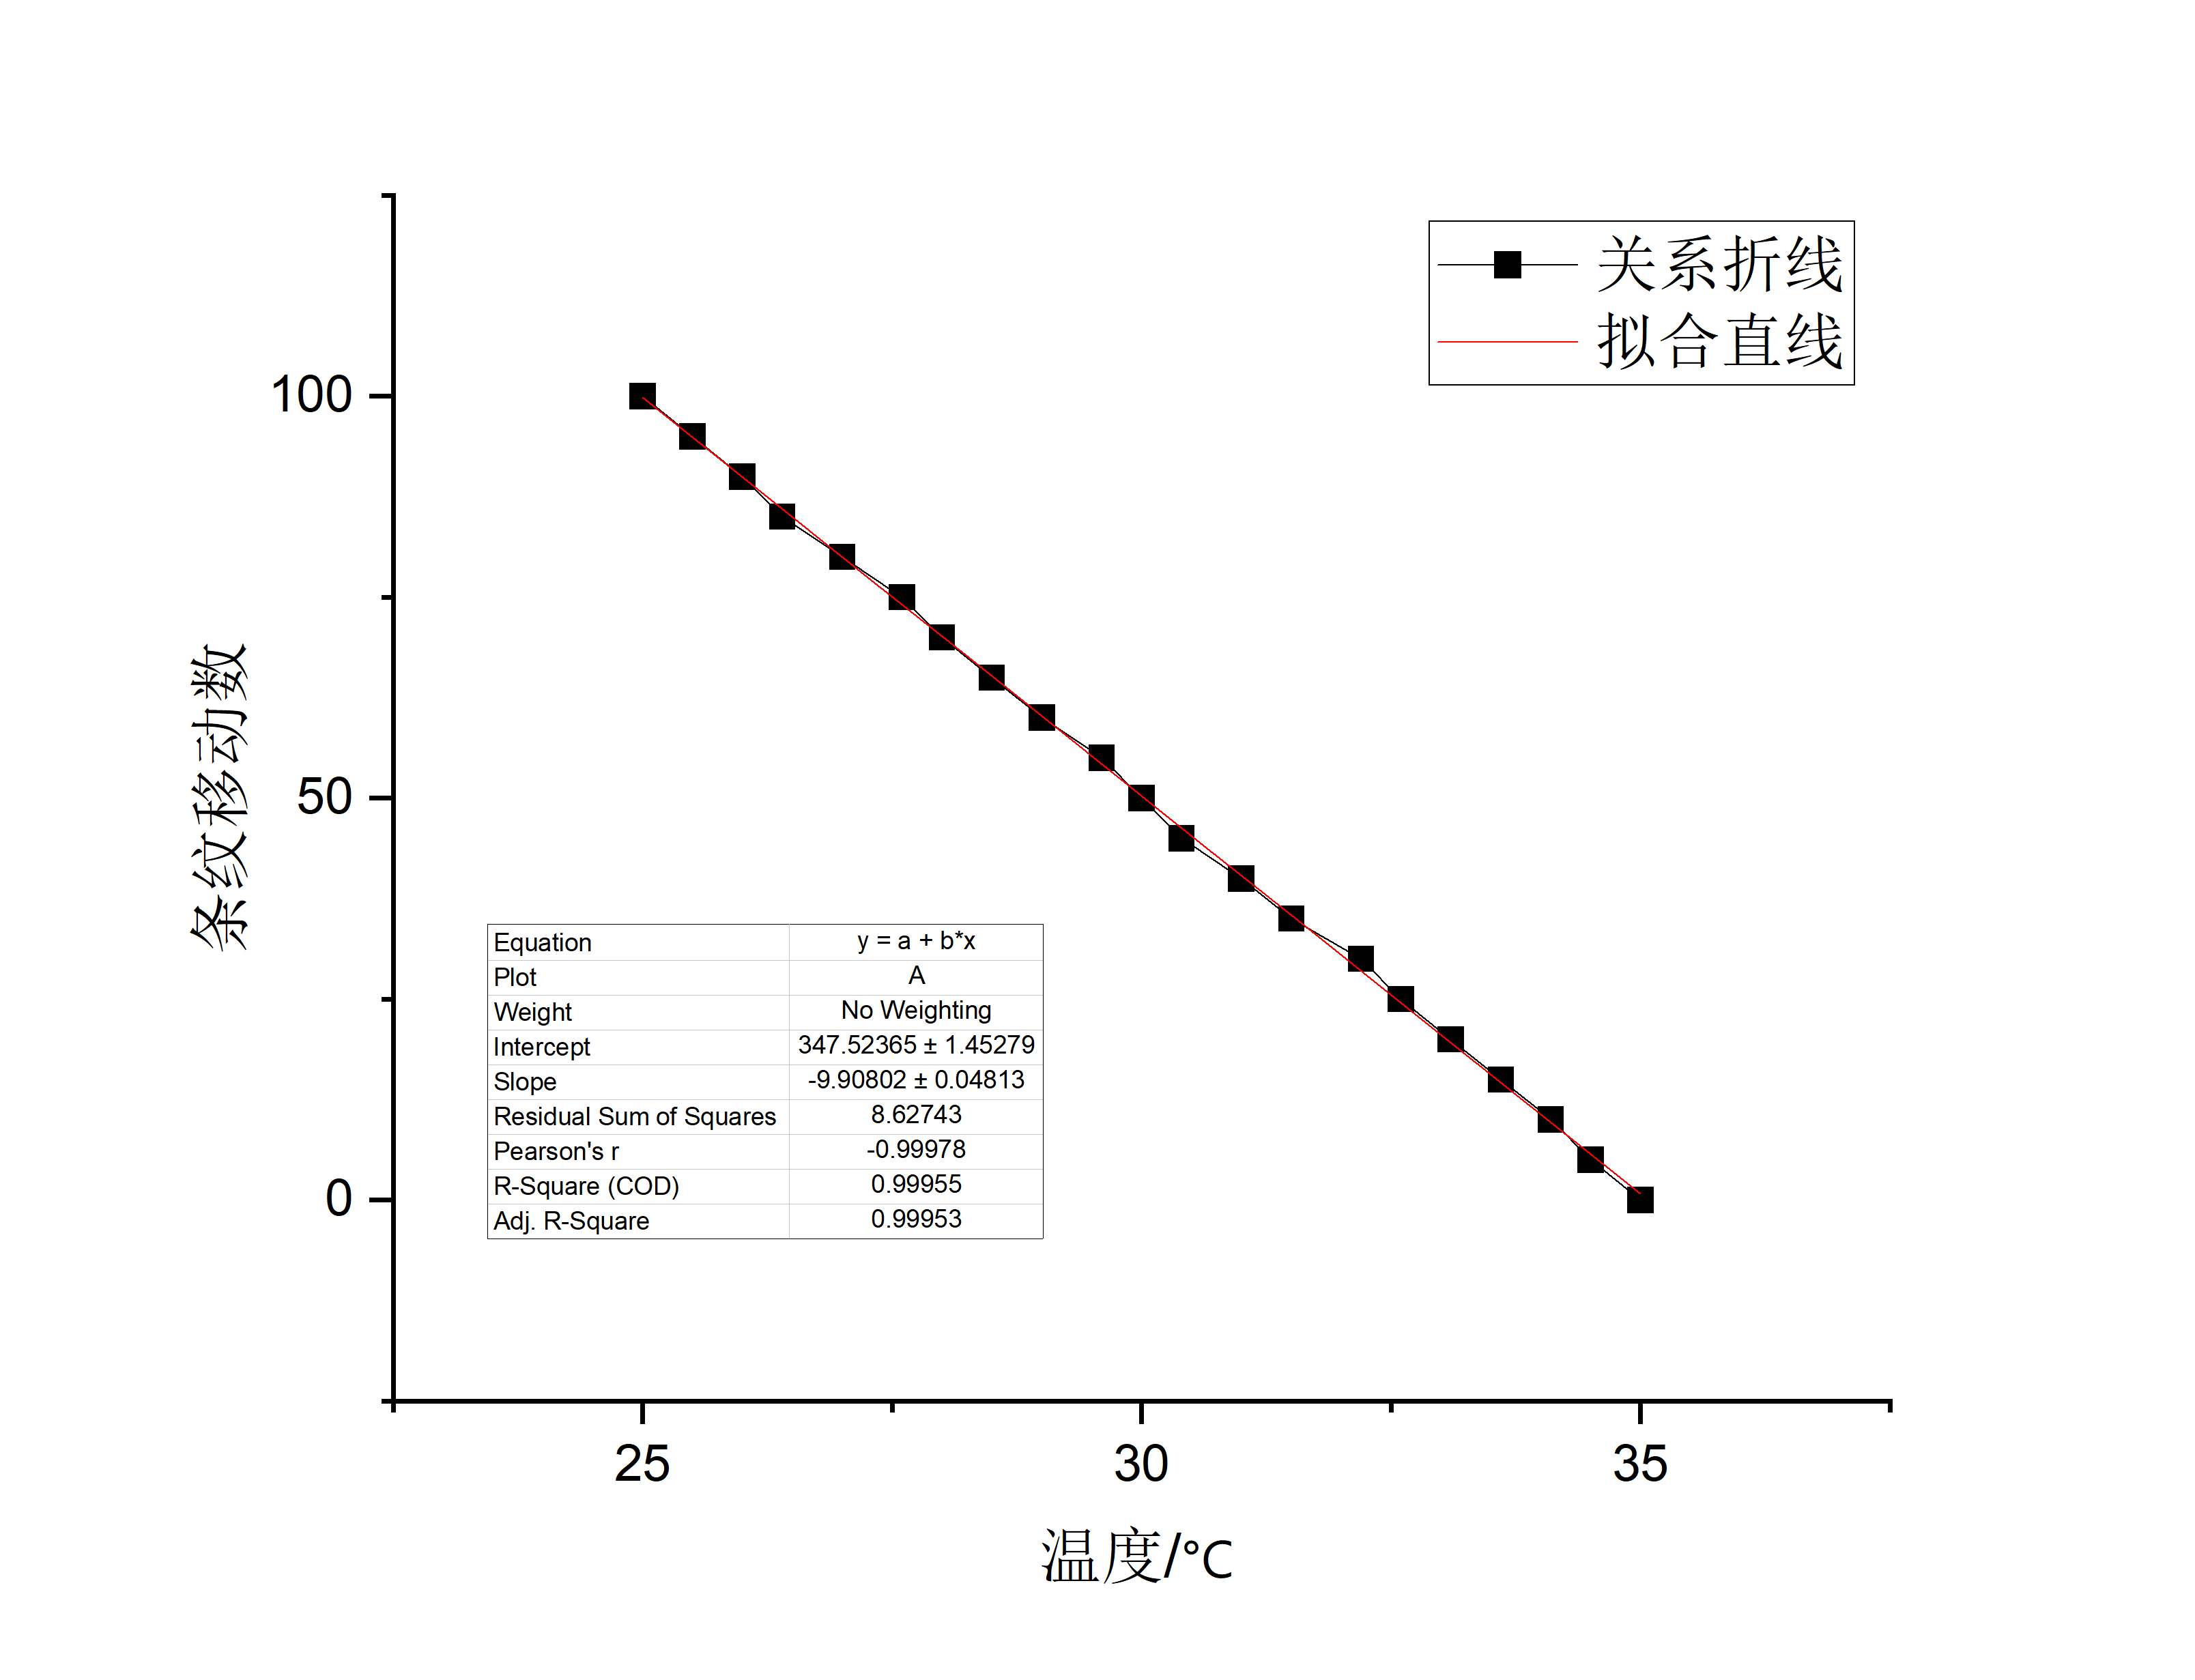
\includegraphics[width=0.48\textwidth]{img//TA2.png}}

	\subfloat[B组上行]{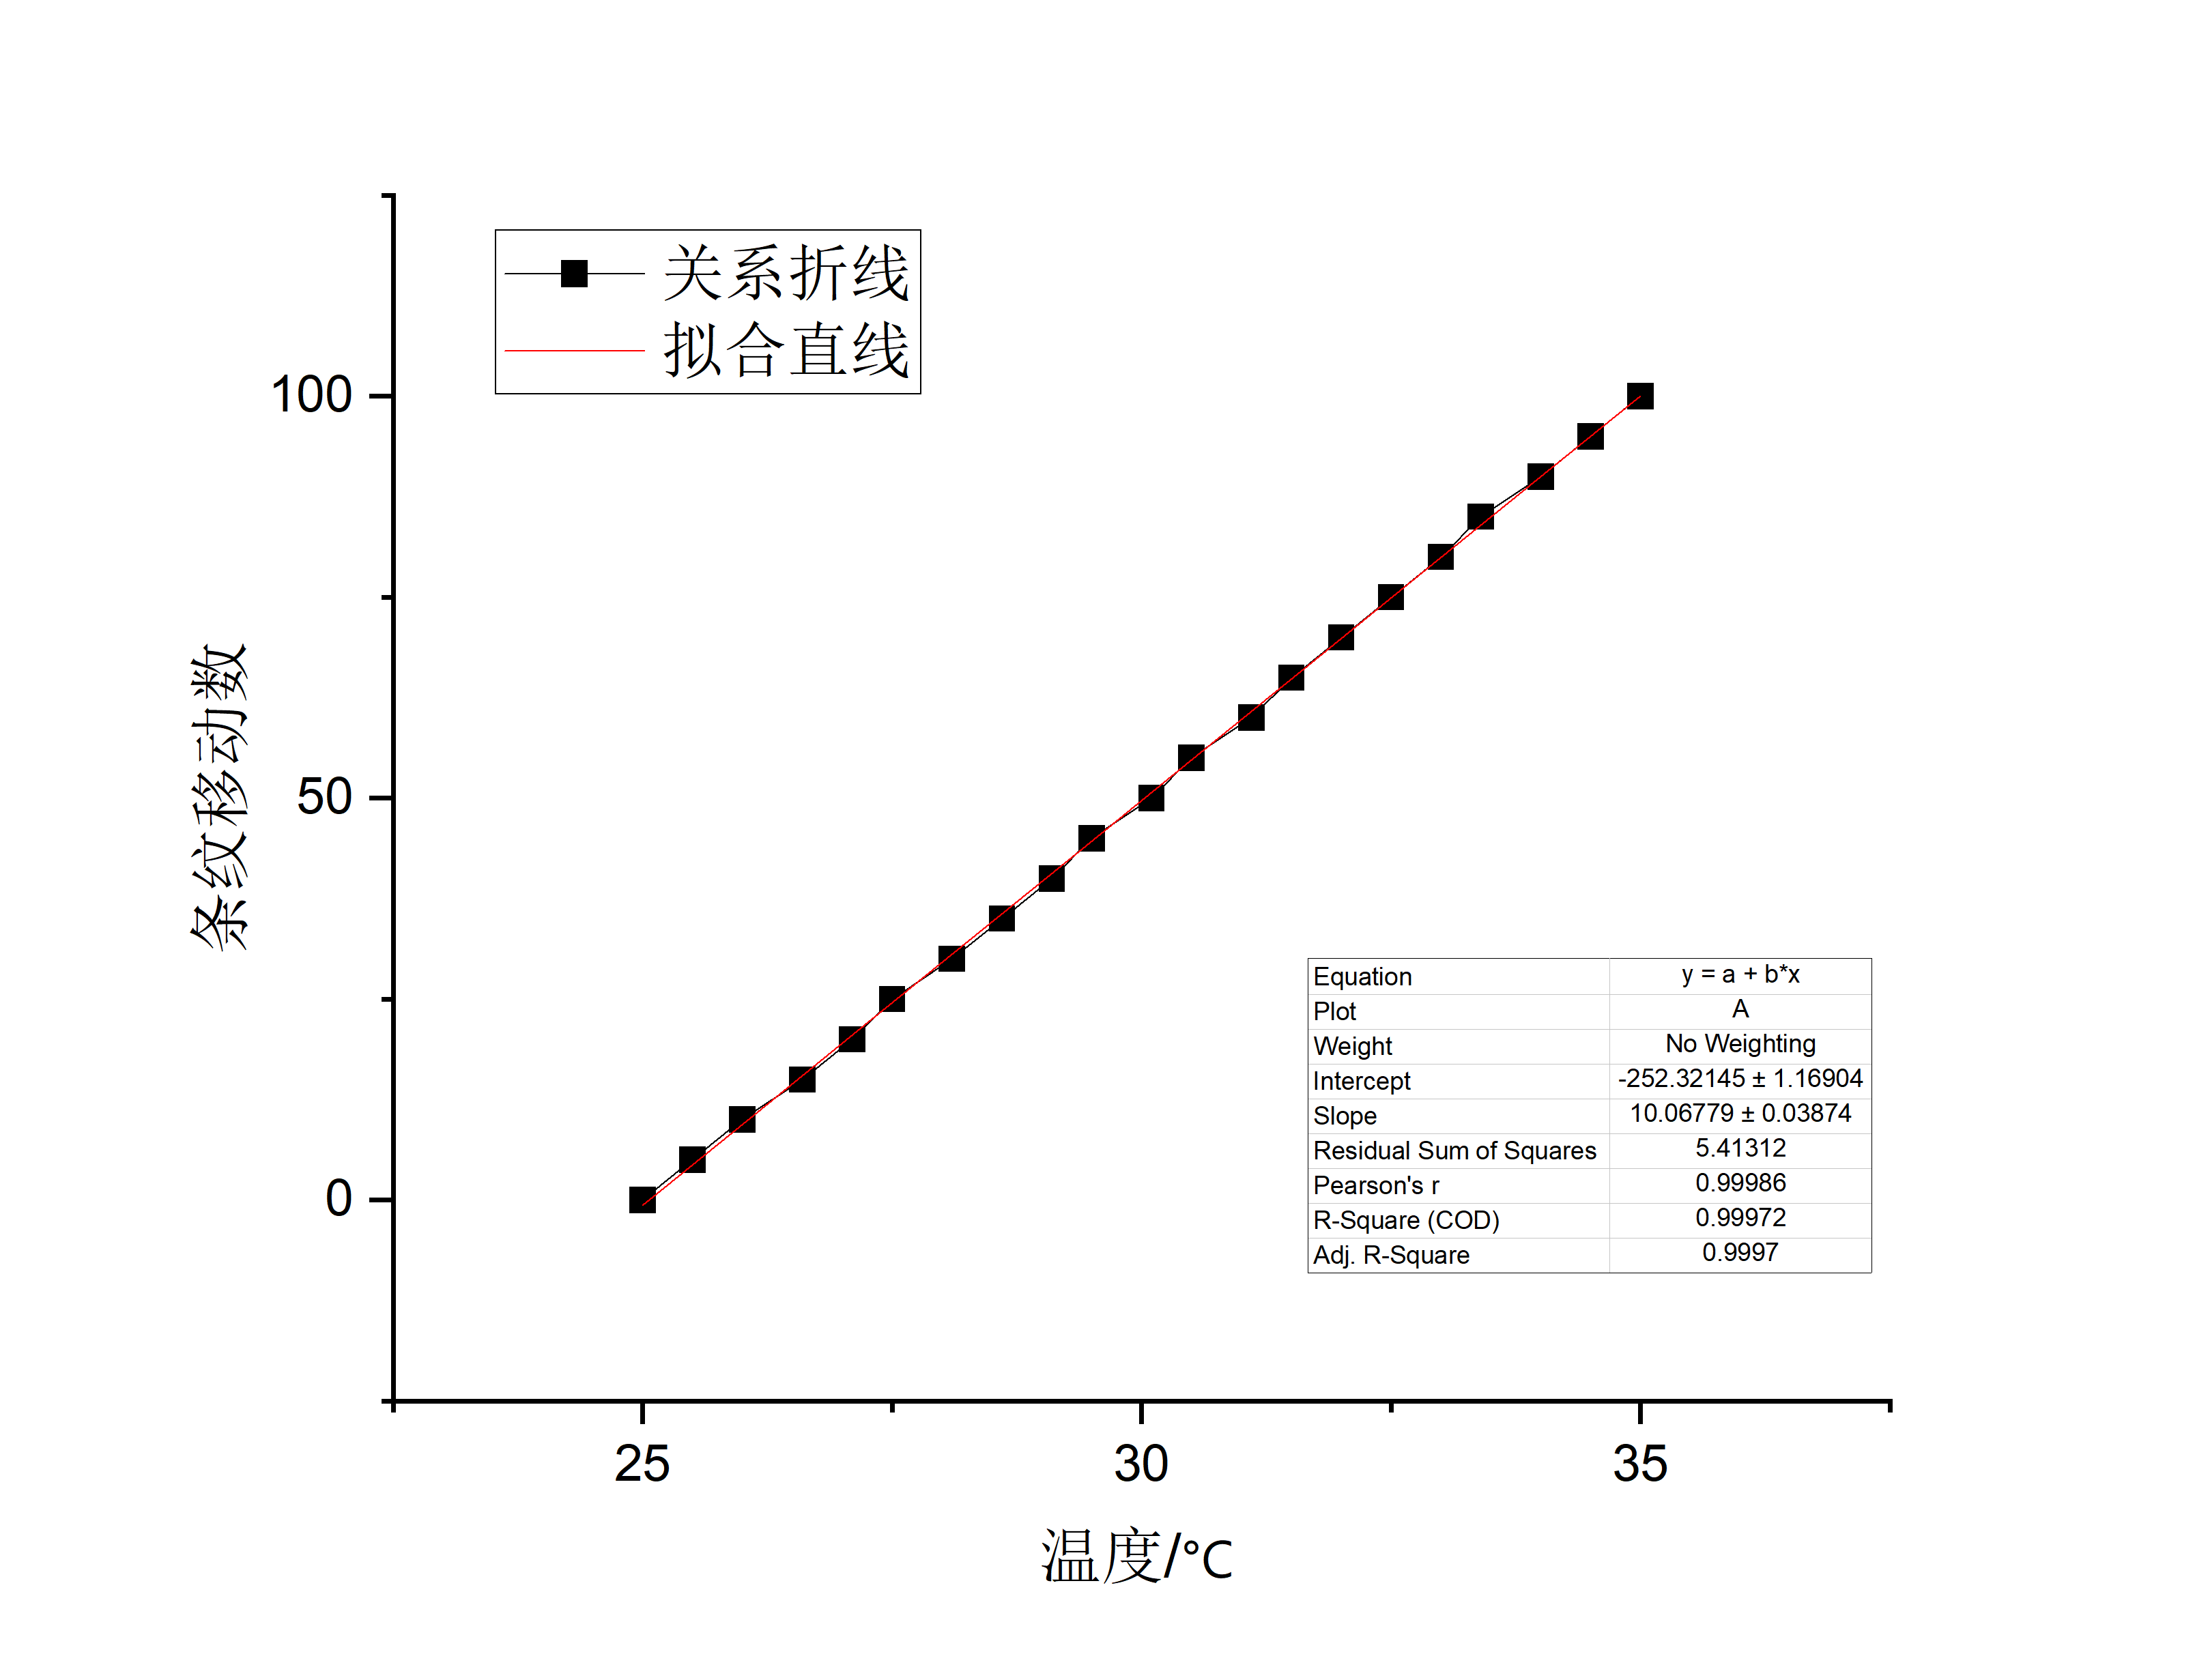
\includegraphics[width=0.48\textwidth]{img//TB1.png}}
	\subfloat[B组下行]{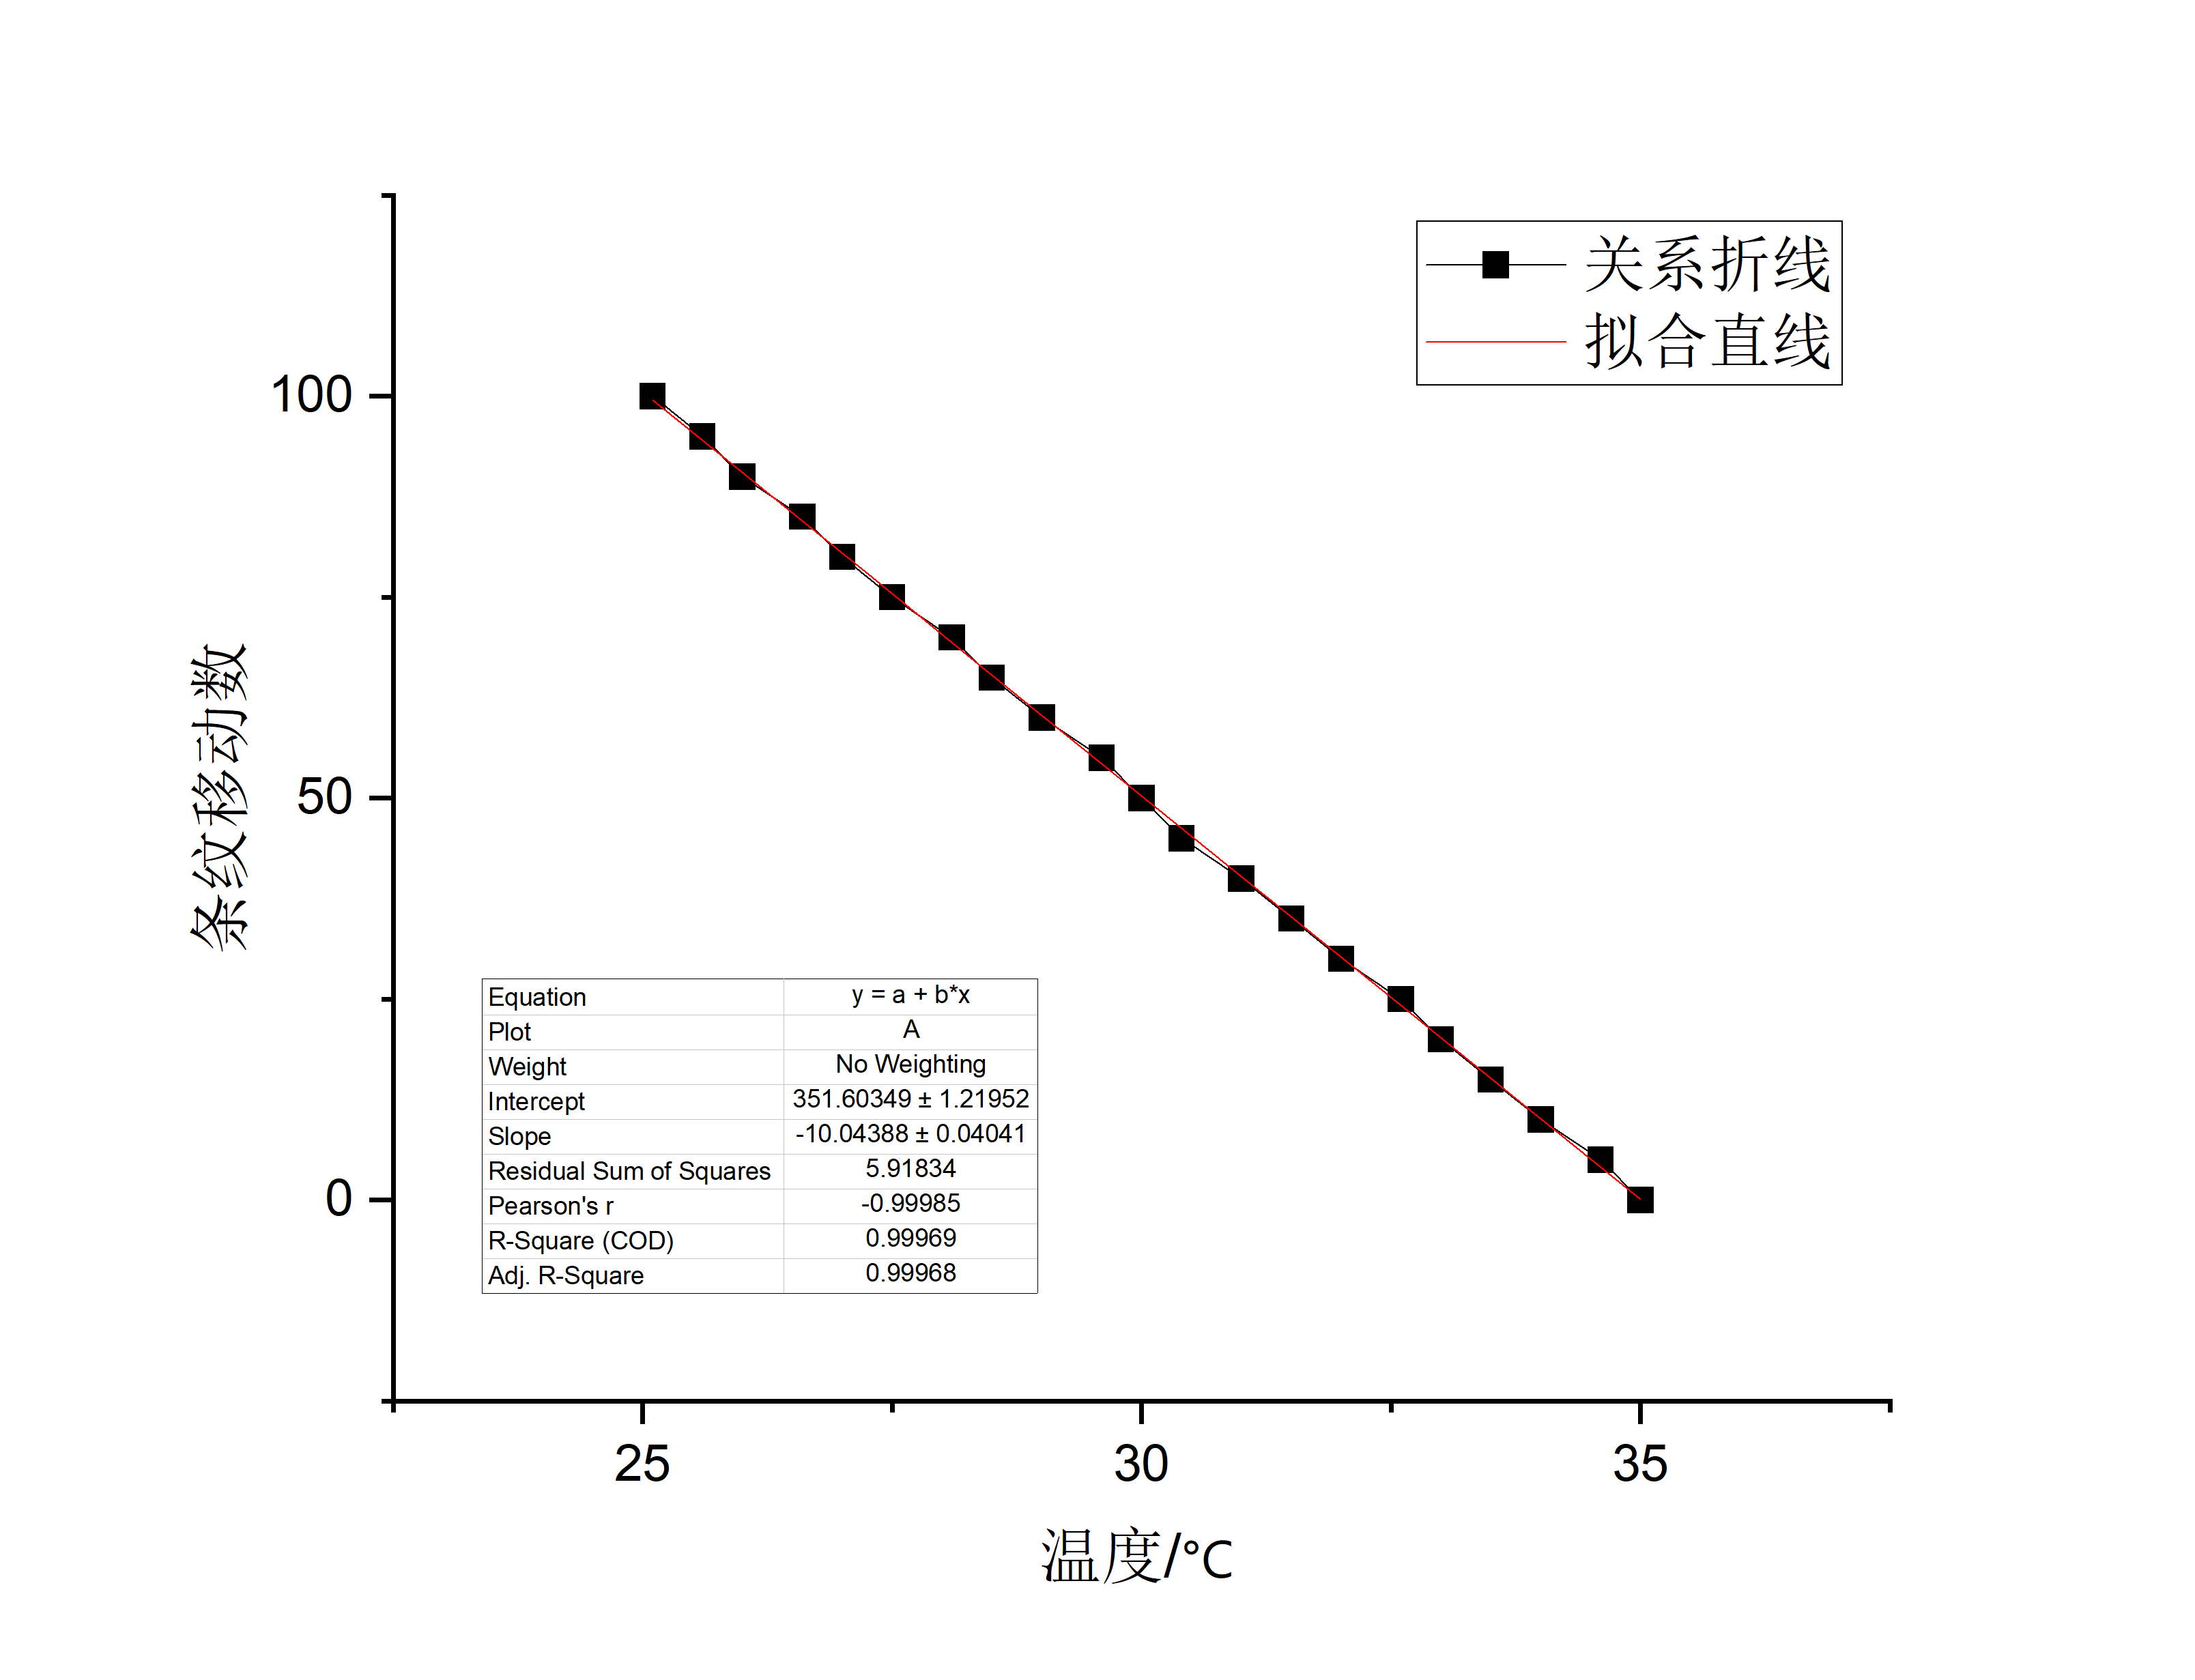
\includegraphics[width=0.48\textwidth]{img//TB2.png}}
	\caption{光纤温度传感器条纹移动数目随温度变化关系}
	\label{fig:T}
\end{figure}

观察实验点的分布可知, 条纹移动数与温度基本上呈线性关系, 进行线性拟合得到直线
相关系数均超过0.99,线性关系成立。 计算得斜率绝对值均值 $\overline{|K|}=10.00 $可知 对于该光纤温度传感器,温度
每增加 1摄氏度, 条纹就会移动 10.00条, 对应的光相位变化$\varDelta \phi=2\pi \varDelta n=62.83rad$ ,
所以, 每升高1摄氏度, 光纤传感器输出光的相位就会变化 62.83rad。


误差分析:
\begin{enumerate}
	\item 条纹存在一定宽度, 无法确认每次计数时条纹处在同一位置。
	\item  条纹十分不易辨识, 容易产生视觉疲劳。
	\item 当停止转动螺杆后, 由于压力回弹, 条纹会反向移动一段距离, 对结果产生影响。
\end{enumerate}

\subsection{光纤偏振光实验}
\subsubsection{线偏振光的斯托克斯参数测量}
在光路中依次放入偏振分光棱镜、偏振片和光探头,偏振分光棱镜方向与图\ref{fig:fenguang}上下相反,以免激光照射到实验人员,后调节元器件使入射平面与平台平行(看反射光是否与出射光光斑重合)。

\begin{figure}[H]
	\centering
	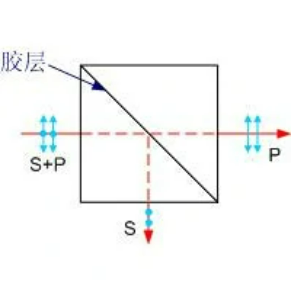
\includegraphics[width=0.3\textwidth]{img//fenguang.png}
	\caption{偏振分光棱镜原理}
	\label{fig:fenguang}
\end{figure}

(1)调节偏振片透光轴与平台水平

粗调偏振片角度,使光功率最大;多次微调偏振片角度,当光功率最大时,
偏振片的轴与平台水平。

(2)调节偏振片透光轴与平台垂直

方法一:粗调偏振片角度,使光功率大致为0;多次微调偏振片角度,此时
偏振片的轴与平台垂直。

方法二:在调节完毕的水平偏振片后放置未调节的垂直偏振片,转动未调节的偏振片至输出光功率最小处(“二分法”),此时第二片偏振片轴与平台垂直。

(3)调节偏振片透光轴与平台成$+45^{\circ}$角

在激光器和调节完成后的水平偏振片后放置待调偏振片,将其按上述方法调节至垂直,迎着光的方向顺时针转动约$45^{\circ}$,细调至出射光功率最大处(马吕斯定律),
此时第二片偏振片与平台成$+45^{\circ}$.


调节完毕后得到三个透光轴分别为水平、垂直以及和平台成$+45^{\circ}$角的偏振片,分别测量激光器对其的透射光功率$P_x$、$P_y$和$P_{+45^{\circ}}$.

为了得到第四个斯托克斯参数,我们要在$+45^{\circ}$线偏振片前面插入快轴与起偏器光轴成45度的
 1/4 波片,测量功率($P_R$)后就能算出第四个斯托克斯参数。


当起偏器光轴为$+45^{\circ}$时,测得$P_x=0.315mW$、$P_y=0.305mW$、$P_{+45^{\circ}}=0.615mW$、$P_R=0.321mW$.

此时有:
\[\left\{
\begin{aligned}
&S_0=P_x+P_y=0.620\\
&S_1=P_x-P_y=0.010\\
&S_2=2P_{+45}-S_0=0.610\\
&S_3=S_0-2P_R=-0.022\\
\end{aligned}
\right.
\]

归一化得斯托克斯矢量:

\begin{equation}
	S=
	\left[ 
		\begin{array}{c}
		1\\
		0.0161\\
		0.9839\\
		-0.0355\\
		\end{array} 
	\right ]
\end{equation}

此时:
\begin{equation*}
	S_1^2+S_2^2+S_3^2=0.96957867
\end{equation*}
计算得偏转角:
\begin{equation*}
	\phi=\frac{1}{2}arctan\left(\frac{S_2}{S_1}\right)=44.5313^{\circ}
\end{equation*}
相对误差为:
\begin{equation*}
	\eta=\frac{45^{\circ}-44.5313^{\circ}}{45^{\circ}}=1.04\%
\end{equation*}

当起偏器光轴为$+65^{\circ}$时,测得$P_x=0.105mW$、$P_y=0.508mW$、$P_{+45^{\circ}}=0.535mW$、$P_R=0.290mW$.

此时有:
\[\left\{
\begin{aligned}
&S_0=P_x+P_y=0.613\\
&S_1=P_x-P_y=-0.403\\
&S_2=2P_{+45}-S_0=0.457\\
&S_3=S_0-2P_R=-0.033\\
\end{aligned}
\right.
\]

归一化得斯托克斯矢量:

\begin{equation}
	S=
	\left[ 
		\begin{array}{c}
		1\\
		-0.6574\\
		0.7455\\
		0.0538\\
		\end{array} 
	\right ]
\end{equation}

此时:
\begin{equation*}
	S_1^2+S_2^2+S_3^2=0.99083945
\end{equation*}
计算得偏转角:
\begin{equation*}
	\phi=\frac{1}{2}arctan\left(\frac{S_2}{S_1}\right)=65.7033^{\circ}
\end{equation*}
相对误差为:
\begin{equation*}
	\eta=\frac{|65^{\circ}-65.7033^{\circ}|}{65^{\circ}}=1.08\%
\end{equation*}


\subsubsection{圆偏振光的斯托克斯参数测量}

产生圆偏振光,即在激光器后放置两个正交的偏振片,在两个偏振片之间放入1/4波片,转动1/4波片使出射光功率最大。
(更精确做法:转动1/4波片找到两个光功率极小值点,此时快慢轴与偏振片正交透射轴重合,记录角度后取中间角度即可产生圆偏振光)

此时转撤去最后一片偏振片,转动检偏器偏器检测到出射光功率应该恒定不变,即1/4波片的出射光为圆偏振光。

多次测定新产生的圆偏振光光功率,按线偏振光的方法测量其斯托克斯矢量。

\[\left\{
\begin{aligned}
&P_x=0.307mW\\
&P_y=0.294mW\\
&P_{+45}=0.312mW\\
&P_R=0.602mW\\
\end{aligned}
\right.
\]

\[\left\{
\begin{aligned}
&S_0=P_x+P_y=0.601\\
&S_1=P_x-P_y=-0.013\\
&S_2=2P_{+45}-S_0=0.317\\
&S_3=S_0-2P_R=-0.613\\
\end{aligned}
\right.
\]

归一化得斯托克斯矢量:

\begin{equation}
	S=
	\left[ 
		\begin{array}{c}
		1\\
		-0.0216\\
		0.5275\\
		-1.0199\\
		\end{array} 
	\right ]
\end{equation}

此时:
\begin{equation*}
	S_1^2+S_2^2+S_3^2=0.1.3189182
\end{equation*}

\subsubsection{光纤出射光斯托克斯参数的测量}
将激光耦合至单模光纤直至功率最大,记录此时光功率,测量斯托克斯矢量,跟之前测量的线偏振光参数对比。用光功率计记录光
强变化曲线,如图\ref{fig:Power},评估实验室使用的非保偏激光器偏振状态的变化情况。


\begin{figure}[H]
	\centering
	\subfloat[$P_x$]{\includegraphics[width=0.35\textwidth]{img//px.jpg}}
	\subfloat[$P_y$]{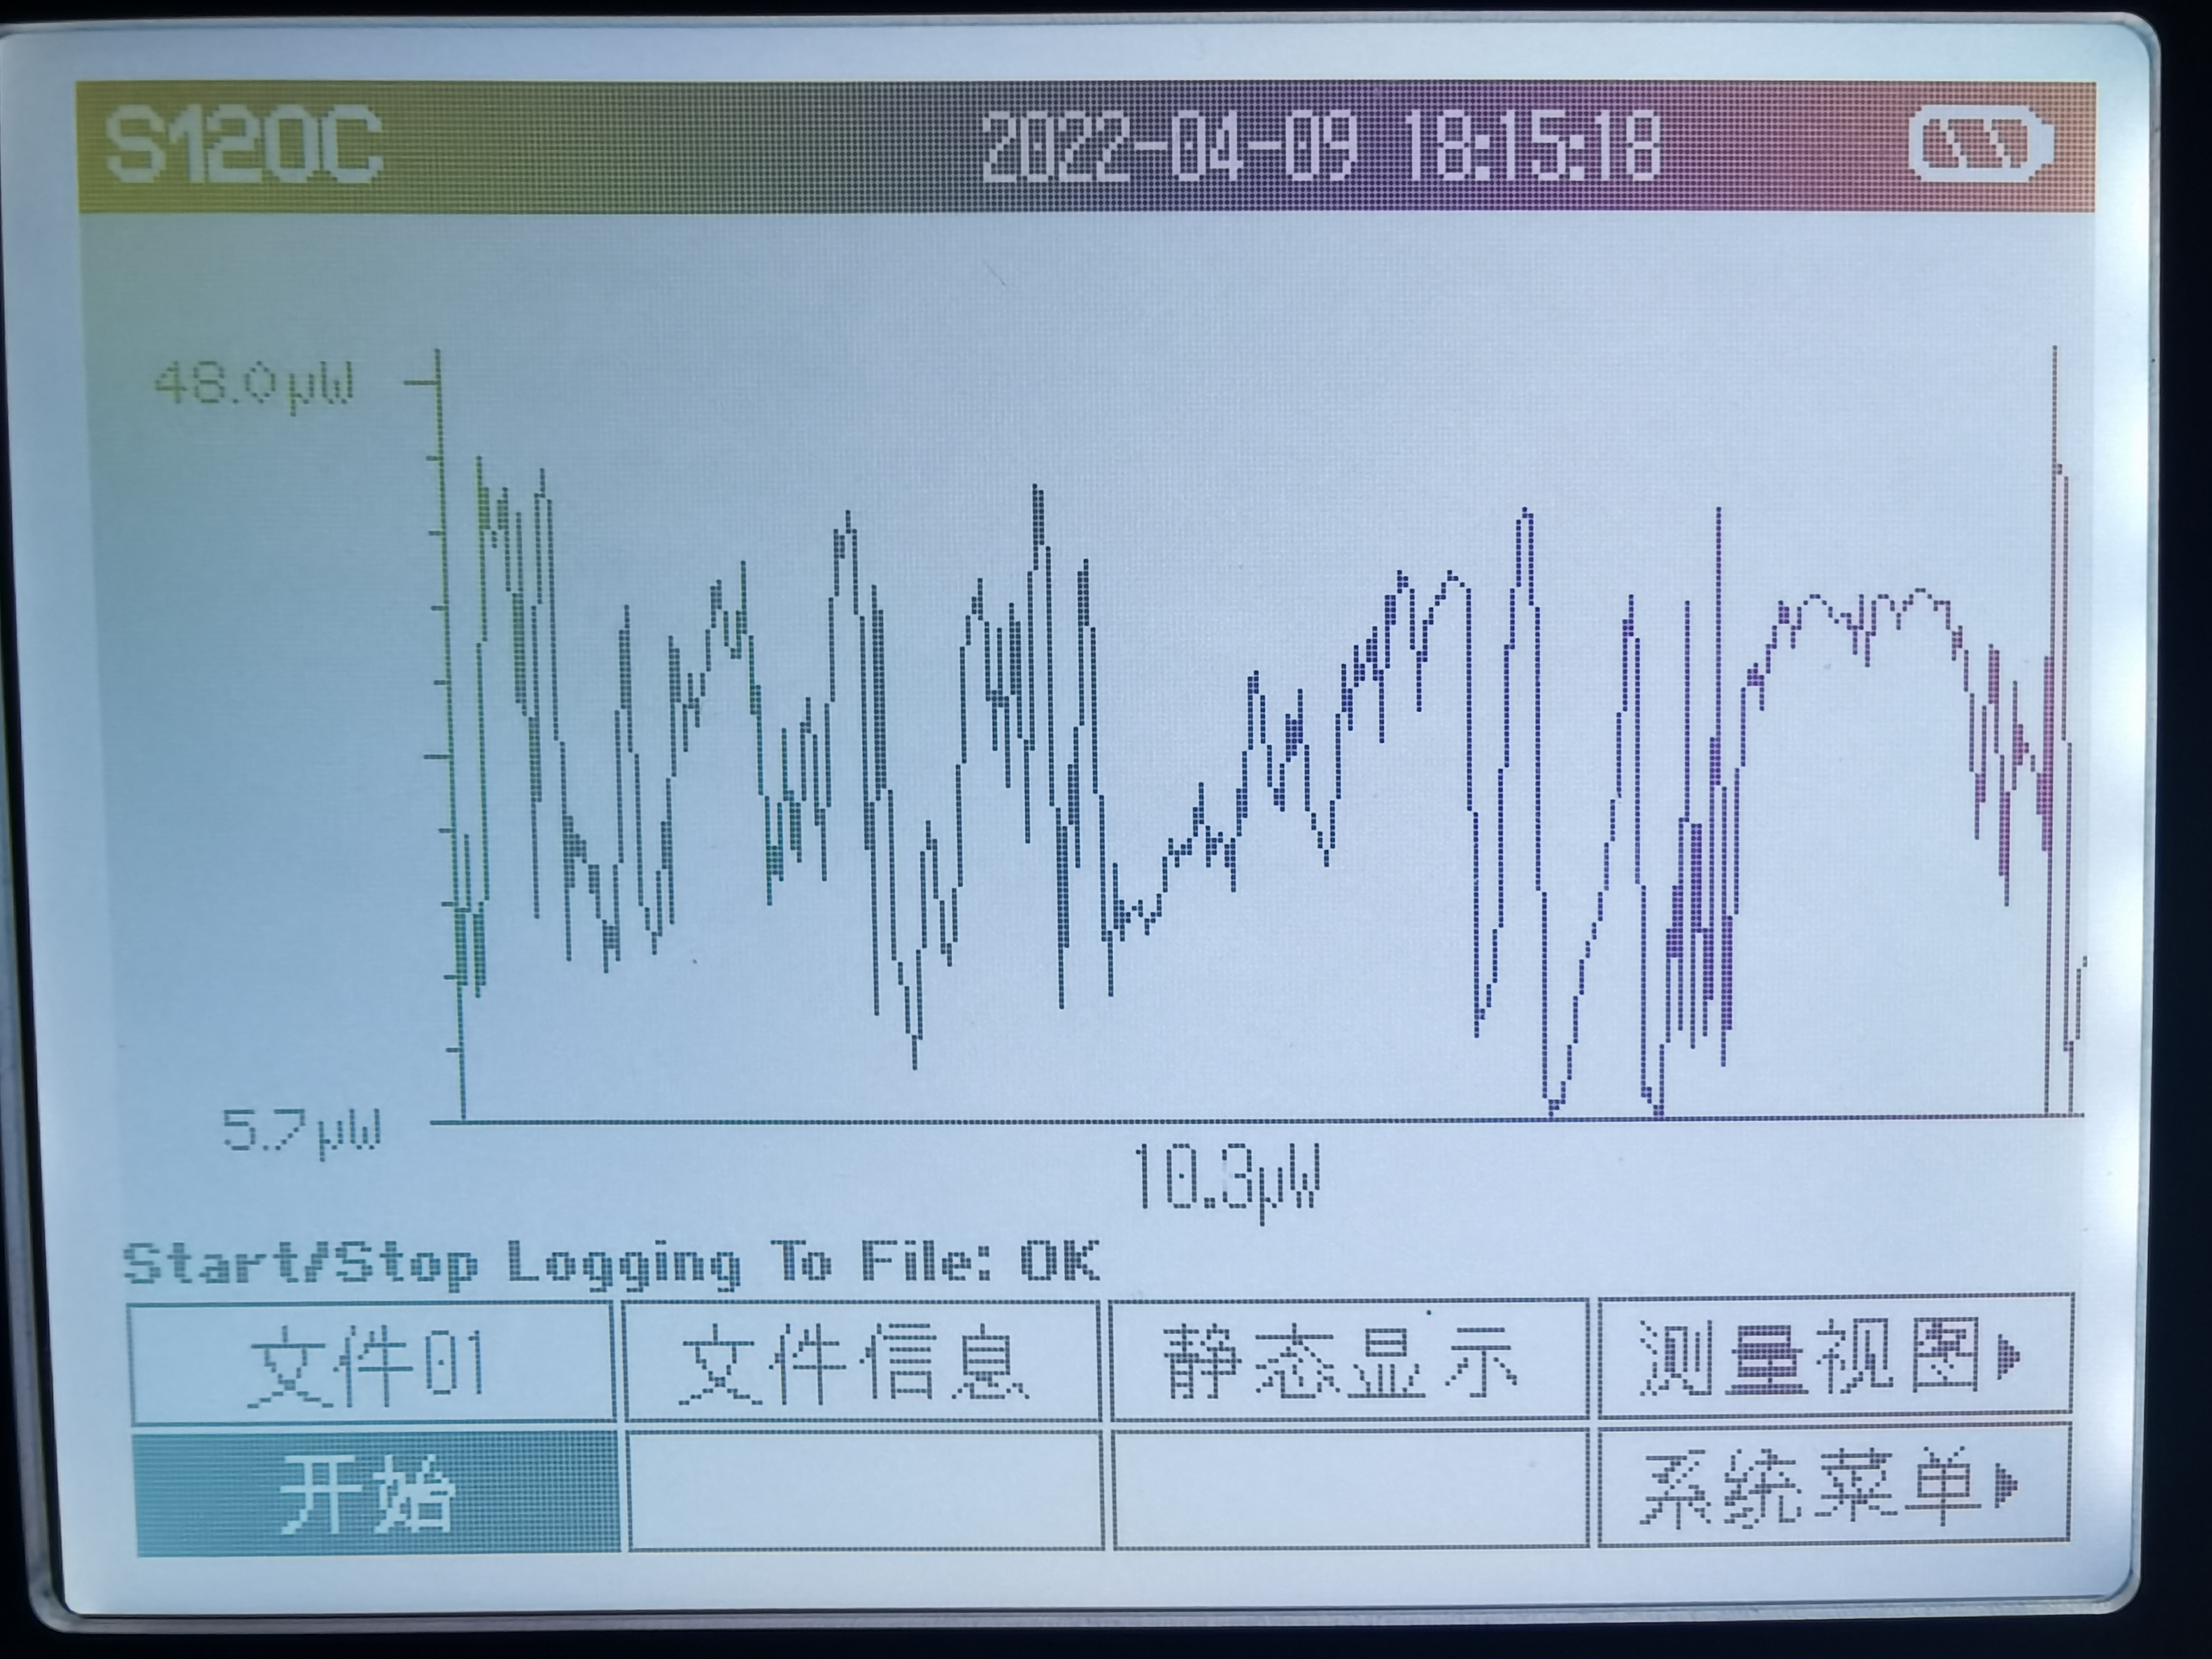
\includegraphics[width=0.35\textwidth]{img//py.jpg}}

	\subfloat[$P_{+45^{\circ}}$]{\includegraphics[width=0.35\textwidth]{img//45.jpg}}
	\subfloat[$P_R$]{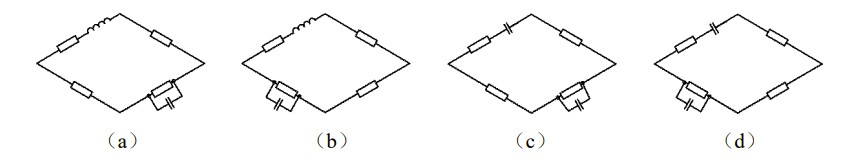
\includegraphics[width=0.35\textwidth]{img//pr.jpg}}
	\caption{光功率随时间变化关系}
	\label{fig:Power}
\end{figure}

由于读数时光功率计示数不恒定,故记录其时域变化曲线。可以看出光功率值波动较大,并且没有收敛值。
鉴于无法同时测量不同方向光功率,故不计算斯托克斯矢量。

\section{讨~~~论}
在光纤光学实验中,粗调透镜至光纤输入端距离,可以发现在调整过程中出现多个峰值,这时找准透镜焦距附近的峰值,即可耦合至光功率最大处。

在光纤压力传感器实验中,一次上行至下行的转换过程中,不可避免螺杆转换转动方向时会有回程误差,多次测量后拟合消减了这部分误差对实验结果的影响。
对于光纤温度传感器,升温时干涉条纹移动不明显,人眼无法对非整数个条纹进行统计,造成误差。其次人眼长时间盯着条纹,视觉上的疲劳影响了判断精度。
由于升温降温的缓慢,本实验最高升温至35摄氏度,若升至更高温度,则可看到更完整的光纤随温度变化特性。

光纤偏振光实验中偏振片本身导致光功率的损耗是一大问题,为了减少损耗,我们尽量减少光程。实验中,线偏振光的斯托克斯参量前三个参数较易测得;
对于圆偏振光来说,实验较难产生标准的圆偏振光。我们检验时发现产生的圆偏振光水平分量和竖直分量上的光功率略有差异,故圆偏振光测量误差大于线偏振光。
当测量光纤耦合后的斯托克斯矢量的时候,我们发现光功率计示数不停变化,且没有收敛的迹象,并且无法同时测量不同偏振方向的光功率,故只测量了光功率时域变化图像。
我们发现一旦光纤输出端与光探头之间超过两个偏振片,由于仪器底座产生的距离使光探头无法覆盖激光光斑,产生大量光功率损耗。

\section{结~~~论}

光纤耦合分为直接耦合和透镜耦合,用同一种耦合方式耦合时,光纤直径越大,其耦合效率越高,传输损耗越低。
将直接耦合方法与透镜耦合方式比较,透镜耦合的效率显著高于直接耦合,并且传输损耗大大降低。这与透镜聚焦,将光功率汇集于焦点的功能息息相关。
测量芯径$4\mu m$,$9\mu m$和$62.5\mu m$光纤的数值孔径分别为$0.0.276556\pm0.005225$,$0.0.276556\pm0.005225$和$0.0.276556\pm0.005225$.

用马赫-曾德尔干涉仪探究应变对光纤的影响,发现条纹移动数与螺旋刻度呈线性关系。计算得斜率绝对值均值 $\overline{|K|}=6.32 $可知 对于该光纤压力传感器, 螺旋
刻度每增加 1mm, 条纹就会移动 6.32 条,对应的光相位变化$\varDelta \phi=2\pi \varDelta n=39.70rad$ ,所以, 每改变螺旋距离 1mm, 光纤传感器输出光的相位就会变化 39.70rad。
探究温度对光纤的影响,发现条纹移动数与温度基本上呈线性关系。计算得斜率绝对值均值 $\overline{|K|}=10.00 $可知 对于该光纤温度传感器,温度
每增加 1摄氏度, 条纹就会移动 10.00条, 对应的光相位变化$\varDelta \phi=2\pi \varDelta n=62.83rad$ ,
所以, 每升高1摄氏度, 光纤传感器输出光的相位就会变化 62.83rad。

最后测得$+45^{\circ}$,$+65^{\circ}$线偏振光和圆偏振光的斯托克斯矢量分别为:
\begin{figure*}[htbp]
	\centering
		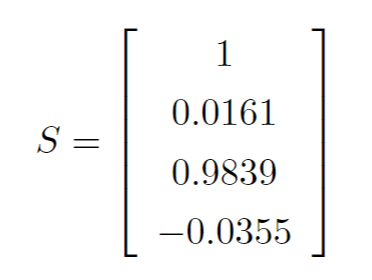
\includegraphics[width=0.2\textwidth]{img//s1.png}
		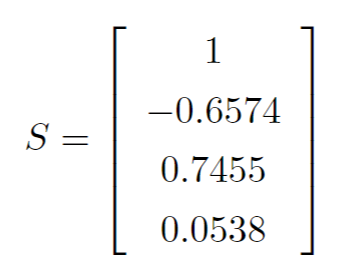
\includegraphics[width=0.2\textwidth]{img//s2.png}
		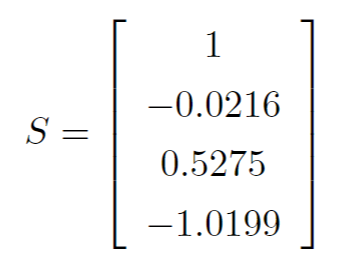
\includegraphics[width=0.2\textwidth]{img//s3.png}
\end{figure*}






\newpage
\section*{参考文献}
% \renewcommand\refname{参考文献}
% \bibliographystyle{chinese}
% \bibliography{ref}

[1] 光纤耦合实验讲义,\url{http://lovephysics.sysu.edu.cn/lib/exe/fetch.php?media=courses:thirdlevel:gpl_iii_south_c6.1_20220210.pdf}.

[2] 光纤传感器实验讲义,\url{http://lovephysics.sysu.edu.cn/lib/exe/fetch.php?media=courses:thirdlevel:gpl_iii_south_c6.2_20220210.pdf}

[3] 光纤的偏振光传输特性实验讲义,\url{http://lovephysics.sysu.edu.cn/lib/exe/fetch.php?media=courses:thirdlevel:gpl_iii_south_c6.3_20220210.pdf}

[4] 陈敏,赵福利,董建文,编著. 光学[M]. 高等教育出版社, 2018. ISBN:9787040489323.

[5] 姜凤贤. 级联光纤光栅传感机理与实验研究[D].燕山大学,2015.

[6] 韩悦文, 陈海燕, 黄春雄:光纤技术在湿度传感器中的应用,TP212. 14;TN818

[7] 任广军,姚建铨,王鹏,张强.保偏光纤激光器的实验研究[J].中国激光,2007(09):1208-1211.


\clearpage

	
\section*{\LARGE 附录A}
\section*{【思考题】}
\subsection*{1. 比较、评估两种耦合方法的耦合效率。}
将直接耦合方法与透镜耦合方式比较,透镜耦合的效率显著高于直接耦合,可知聚焦透镜耦合比直接耦合效果好得多。
这与透镜聚焦,将光功率汇集于焦点的功能息息相关。

\subsection*{2. 计算耦合效率(结果用 dB 表示),对自己的工作进行评估。}
由实验结果可知,芯径$4\mu m、9\mu m、62.5\mu m$光纤直接耦合效率为45.06DdB、40.82dB、25.21dB;间接耦合效率分别为3.42dB、1.46dB、1.32dB。

评估: 实验结果初步符合预期实验结果,但仍有改进的空间。存在的误差可能有:
\begin{enumerate}
	\item 光功率计的读数存在较大的跳动, 可能会导致输出端光功率和激光器光功率的测量存在误差。
	\item 光纤在使用的过程中, 操作不当导致的光纤非自然弯曲可能影响示数
	\item 光纤切面端口不平整,反射过大造成的误差
	\item 实验中, 光线与激光光源很难完全耦合, 存在光路并非准直的可能
	\item 空气温度、湿度造成的误差
\end{enumerate}

\subsection*{3. 以你实验后的认识写下单模、多模光纤之间的区别。}
单模光纤中只能传导一种模式的光波, 多模光纤中可以传导多种模式的光波。 实验中发
现多模光纤的耦合效率比单模光纤要好, 可能使因为多模光纤可以传导多种模式的光波,
没有单模中的损耗, 使得传输效率较高。

\subsection*{4. 查阅资料,了解几种光纤传感器的类型,简要写出工作原理。}
(1)光纤光栅传感器

当光纤光栅所处环境的温度、应力、应变或其它物理量发生变化时,光栅的周期或纤芯折射率将发生变化,从而使反射光的波长发生变化。
通过测量物理量变化前后反射光波长的变化,就可以获得待测物理量的变化情况。
如利用磁场诱导的左右旋极化波的折射率变化不同,可实现对磁场的直接测量。
此外,通过特定的技术,可实现对应力和温度的分别测量,也可同时测量。
通过在光瓯上涂敷特定的功能材料(如压电材料),还可实现对电场等物理量的间接测量。

(2)长周期光纤光栅(LPG)传感器

长周期光纤光册(LPG)的周期一般认为有数百微米,LPG在特定的波长上把纤芯的光耦合进包层。
光在包层中将由于包层/空气界面的损耗而迅速衰减,留下一串损耗带。
一个独立的LPG可能在一个很宽的波长范围上有许多的共振,LPG共振的中心波长主要取决于芯和包层的折射率差,
由应变、温度或外部折射率变化而产生的任何变化都能在共振中产生大的波长位移,通过检测$\varDelta X_i$,就可获得外界物理量变化的信息。
LPG在给定波长上的共振带的响应通常有不同的幅度,因而LPG适用于多参数传感器。

(3)光纤光栅式湿度传感器

对温度、 湿度敏感的光线布拉格光栅 FBG1 和仅对温度敏感的 FBG2 串联构成。 FBG1 的涂覆
层为改良聚酰亚胺(PI)湿敏薄膜。 湿度和温度的变化使 FBG 的布拉格反射波长入 p1 和入
p2 发生漂移。 变化量分别为 AA, 和 AA2, 由此可计算出温度、 湿度的变化值。



\subsection*{5. 光纤偏振光的实验结果与斯托克斯矢量公式对比,分析误差产生的原因。}
\begin{enumerate}
	\item 激光器产生的功率不能保持恒定不变,故不同时间测得的光功率组合成斯托克斯矢量存在偏差
	\item 光通过偏振片存在损耗
	\item 光在偏振片之间会有(多次)反射,如果未将入射平面调水平,光路调至直线,将损耗一部分光功率
	\item 光纤耦合时并不能耦合至最佳效果,有微小扰动都会影响耦合效率
	\item 光探头距光纤出射端由于加了偏振片而变远,导致光斑过大,光探头探测面并不能覆盖整个光斑 
\end{enumerate}

\subsection*{6. 检索资料,说明保偏激光如何稳定输出光的偏振状态.}
光纤激光器以其结构简单紧凑 、体积小、工作稳
定可靠、无须调试、光束质量好 、易于集成等特点, 一
直被人们认为是固体激光技术实用化的最佳选择。
保偏光纤是在单模光纤纤芯的两侧加上足够的应
力,使光纤在截面上的两互相垂直方向上产生大的
传播常数差,也即高的双折射,从而实现其保偏性
能。保偏光纤主要结构有:熊猫型光纤,
领结型光纤,椭圆包层型光纤,椭圆芯光纤等,其中
熊猫型保偏光纤因具备诸多优点而深得用户青睐。
人们通常采用保偏光纤和附加的偏振器件共同作
用,或者在光纤上刻蚀布拉格光栅作为偏振选择元
件的手段来实现保偏光纤激光器。

\end{document}
